\documentclass{beamer}
\usepackage{booktabs}
\usepackage{pdfpages}
\usepackage{mathtools}
\usepackage{enumerate}
\usepackage{multirow,tabularx}
\usepackage{booktabs}
\usepackage{pdfpages}
\usepackage{proof}
\usepackage{cancel}
\usepackage{chronology}
\usepackage{graphicx}
\usepackage{ulem}
\usepackage{amsmath}
\usepackage{amssymb}
\usepackage{color}
\usepackage{animate}

\PassOptionsToPackage{usenames,dvipsnames,svgnames}{xcolor}  
\usepackage{tikz}
\usepackage{tkz-graph}


\usepackage{wasysym}
\usepackage{proof}
\usepackage{cancel}
\usepackage{chronology}
\usepackage{graphicx}
\usepackage{ulem}
\usepackage{amsmath}
\usepackage{amssymb}
\usepackage{color}
\usepackage{xcolor}
\usepackage{soul}
%\usepackage{pstricks}
\setbeamertemplate{navigation symbols}{}

\newcommand{\norm}[1]{\left\lVert#1\right\rVert}
\newcommand{\el}{$\mathcal{EL}^{++}$}
\renewcommand{\Re}{\mathbb{R}}
\newcommand{\BigO}[1]{\ensuremath{\operatorname{O}\bigl(#1\bigr)}}
\newcommand{\myul}[2][blue]{\sethlcolor{#1}\hl{#2}\setulcolor{black}}

\newcommand<>{\cunderline}[3]{\only<#1>{#3}\only<#2>{\underline{#3}}}
\newcommand<>{\cem}[3]{\only<#1>{#3}\only<#2>{\ul{#3}}}
\newcommand<>{\cgray}[3]{\only<#1>{#3}\only<#2>{\textcolor{gray}{#3}}}
\newcommand<>{\colorize}[4]{\only<#1>{#4}\only<#2>{\textcolor{#3}{#4}}}

%\setbeamertemplate{navigation symbols}{}
\addtobeamertemplate{navigation symbols}{}{%
    \usebeamerfont{footline}%
    \usebeamercolor[fg]{footline}%
    \hspace{1em}%
    \insertframenumber/\inserttotalframenumber
}

\renewcommand{\em}{\itshape}

\mode<presentation>
% {
%   \usecolortheme{crane}
% %  \usetheme{Frankfurt}
% }
\mode<presentation>
{
  \usecolortheme{dove}
}

% \mode<presentation>
% {
% \useinnertheme[shadow=true]{rounded}
% \useoutertheme{infolines}
% \usecolortheme{dove}
% \setbeamerfont{block title}{size={}}
% }

\title[Bio-Ontologies]{Machine learning with ontologies}

\author{Robert Hoehndorf}


\date{}

\begin{document}

\begin{frame}
  \titlepage
\end{frame}

% What ontologies are

% How to find ontology => excercise

% Axioms in ontologies => excercise in AberOWL

% OWL basics, and reasoning; OBO-style and OWL-style identifiers

% How ontologies are used; Gene Ontology; Phenotypes => excercise:
% find annotations


\begin{frame}
\frametitle{Overview}
\tableofcontents
\end{frame}

\section{Ontologies and graphs}

\begin{frame}
  \frametitle{Ontologies, axioms, and bioinformatics}
  \begin{itemize}
  \item ontologies are ubiquitous
  \item rich formal characterization (axioms)
  \item how can they be used for (predictive) data analysis?
    \begin{itemize}
    \item ``fuzzy'', similarity-based search
    \item predictive analysis and machine learning
    \end{itemize}
  \end{itemize}
\end{frame}

\begin{frame}
  \frametitle{Agenda}
  \begin{itemize}
  \item Introduction
  \item Ontologies, graphs, axioms, reasoning
  \item Semantic similarity
  \item Machine learning
  \end{itemize}
\end{frame}

\begin{frame}
  \frametitle{Preliminaries: ontologies}
  \begin{itemize}
  \item Specific artifacts expressing the intended meaning of a
    vocabulary in terms of primitive categories and relations
    describing the nature and structure of a domain of discourse
    \begin{itemize}
    \item in order to account for the competent use of vocabulary in
      real situations (such as annotations in databases, etc.)
    \end{itemize}
    \pause
  \item the intended meaning of {\em primitive} categories and
    relations is expressed through axioms (axiomatic method, Tarski)
  \end{itemize}
\end{frame}

\begin{frame}
  \frametitle{Preliminaries: axioms}
  \begin{itemize}
  \item {\em classes} represent kinds of things in the world
    \begin{itemize}
    \item {\em Arm}, {\em Apoptosis}, {\em Influenza}, {\em Homo
        sapiens}, {\em Drinking behavior}, {\em Membrane}
    \end{itemize}
    \pause
  \item {\em instances} of classes are individuals satisfying the
    classes' intension
    \begin{itemize}
    \item my arm, the influenza I had last year, one ethanol molecule, etc.
    \end{itemize}
    \pause
  \item {\em relations} between instances arise from interactions,
    configurations, etc., of individuals
    \begin{itemize}
    \item my arm is {\bf part of} me, the {\bf duration of} my
      influenza was 10 days
    \end{itemize}
    \pause
  \item {\em axioms} specify the conditions that instances of a class
    must satisfy
    \begin{itemize}
    \item every instance of {\em Hand} is a {\bf part of} an instance
      of {\em Arm}
    \end{itemize}
  \end{itemize}
\end{frame}

\begin{frame}
  \frametitle{Description Logics: overview}
  \begin{itemize}
  \item TBox: axioms pertaining to the terminology of the domain (classes)
  \item ABox: axioms stating facts (assertions) about the world
  \item RBox: axioms holding for relations
    \pause
  \item Reasoning: derive implicitly represented knowledge (e.g.,
    subsumption)
  \end{itemize}
\end{frame}

\begin{frame}
  \frametitle{Description Logic ALC: syntax}
  \begin{definition}
    Let $N_C$ be a set of concept names and $N_R$ be a set of relation
    names, $N_C \cap N_R = \emptyset$. $\mathcal{ALC}$ concept
    descriptions are inductively defined as:
    \begin{itemize}
    \item If $A \in N_C$, then $A$ is an $\mathcal{ALC}$ concept
      description
    \item If $C, D$ are $\mathcal{ALC}$ concept description, and $r
      \in N_R$, then the following are $\mathcal{ALC}$ concept descriptions:
      \begin{itemize}
      \item $C \sqcap D$
      \item $C \sqcup D$
      \item $\neg C$
      \item $\forall r.C$
      \item $\exists r.C$
      \end{itemize}
    \end{itemize}
  \end{definition}
  \begin{itemize}
  \item Use $\bot$ as abbreviation of $A \sqcap \neg A$, $\top$ as
    abbreviation of $A \sqcup \neg A$
  \end{itemize}
\end{frame}
% Examples of concept descriptions, dl1.pdf, p8

\begin{frame}
  \frametitle{Description Logic ALC: semantics}
  \begin{definition}
    An interpretation
    $\mathcal{I} = (\Delta^\mathcal{I}, \cdot^\mathcal{I})$ consists
    of a non-empty domain $\Delta^\mathcal{I}$ and an interpretation
    function $\cdot^\mathcal{I}$:
    \begin{itemize}
    \item $A^\mathcal{I} \subseteq \Delta^\mathcal{I}$ for all $A \in
      N_C$,
    \item $r^\mathcal{I} \subseteq \Delta^\mathcal{I} \times
      \Delta^\mathcal{I}$ for all $r \in N_R$
    \end{itemize}
    The interpretation function is extended to $\mathcal{ALC}$ concept
    descriptions as follows:
    \begin{itemize}
    \item $(C \sqcap D)^\mathcal{I} := C^\mathcal{I} \cap D^\mathcal{I}$
    \item $(C \sqcup D)^\mathcal{I} := C^\mathcal{I} \cup D^\mathcal{I}$
    \item $(\neg C)^\mathcal{I} := \Delta^\mathcal{I} - C^\mathcal{I}$
    \item $(\forall r.C)^\mathcal{I} := \{ d \in \Delta^\mathcal{I} |
      \mbox{for all } e \in \Delta^\mathcal{I}: (d,e) \in
      r^\mathcal{I} \mbox{ implies } e \in C^\mathcal{I}\}$
    \item $(\exists r.C)^\mathcal{I} := \{ d \in \Delta^\mathcal{I} |
      \mbox{there is } e \in \Delta^\mathcal{I}: (d,e) \in
      r^\mathcal{I} \mbox{ and } e \in C^\mathcal{I}\}$
    \end{itemize}
  \end{definition}
\end{frame}

\begin{frame}
  \frametitle{Description Logic: terminologies}
  \begin{itemize}
  \item A concept definition is of the form $A \equiv C$ where
    \begin{itemize}
    \item $A$ is a concept name
    \item $C$ is a concept description
    \end{itemize}
  \item A TBox is a finite set of concept definitions such that it
    \begin{itemize}
    \item does not contain multiple definitions, % A equiv B, A equiv C
    \item does not contain cyclic definitions
      % A equiv B and C, B equiv A and C
    \end{itemize}
  \item A {\em defined concept} occurs on the left-hand side of a
    definition
  \item A {\em primitive concept} does not occur on the left-hand side
    of a definition
    % See: axiomatic-deductive method!
  \item An interpretation $\mathcal{I}$ is a model of a TBox
    $\mathcal{T}$ if it satisfies all its concept definitions:
    $A^\mathcal{I} = C^\mathcal{I}$ for all $A \equiv C \in \mathcal{T}$
  \end{itemize}
\end{frame}

\begin{frame}
  \frametitle{Description Logic: assertions}
  \begin{itemize}
  \item An assertion is of the form $C(a)$ (concept assertion) or
    $r(a,b)$ (role assertion), where $C$ is a concept description, $r$
    is a role, $a,b$ are individual names from a set $N_I$ of such
    names
  \item An ABox is a finite set of assertions
  \item An interpretation $\mathcal{I}$ is a model of an ABox
    $\mathcal{A}$ if it satisfies all its assertions:
    \begin{itemize}
    \item $a^\mathcal{I} \in C^\mathcal{I}$ for all $C(a) \in
      \mathcal{A}$
    \item $(a^\mathcal{I},b^\mathcal{I}) \in r^\mathcal{I}$ for all
      $r(a,b) \in \mathcal{A}$
    \end{itemize}
  \end{itemize}
\end{frame}


\begin{frame}
  \frametitle{Description Logic: Reasoning}
  \begin{itemize}
  \item Subsumption: Is $C$ a subconcept of $D$?
    \begin{itemize}
    \item $C \sqsubseteq_\mathcal{T} D$ iff $C^\mathcal{I} \subseteq
      D^\mathcal{I}$ for all models $\mathcal{I}$ of $\mathcal{T}$
    \end{itemize}
  \item Satisfiability: Is the concept $C$ non-contradictory?
    \begin{itemize}
    \item $C$ is satisfiable w.r.t. $\mathcal{T}$ iff $C^\mathcal{I}
      \not= \emptyset$ for some model $\mathcal{I}$ of $\mathcal{T}$
    \end{itemize}
  \item Consistency: Is the ABox $\mathcal{A}$ non-contradictory?
    \begin{itemize}
    \item $\mathcal{A}$ is consistent w.r.t. $\mathcal{T}$ iff it has
      a model that is also a model of $\mathcal{T}$
    \end{itemize}
  \item Instantiation: Is $e$ an instance of $C$?
    \begin{itemize}
    \item $\mathcal{A} \models_\mathcal{T} C(e)$ iff $e^\mathcal{I}
      \in C^\mathcal{I}$ for all models $\mathcal{I}$ of $\mathcal{T}$
      and $\mathcal{A}$.
    \end{itemize}
  \end{itemize}
\end{frame}

\begin{frame}
  \frametitle{Ontologies provide background knowledge}
  \centerline{\includegraphics[width=.8\textwidth]{t-cell-aggregation.png}}
\end{frame}

\begin{frame}
  \frametitle{Ontologies provide background knowledge}
  \centerline{\includegraphics[width=.8\textwidth]{t-cell-activation.png}}
\end{frame}

\begin{frame}
  \frametitle{Ontologies provide background knowledge}
  \centerline{\includegraphics[width=.95\textwidth]{moesin-1.png}}
  \centerline{\includegraphics[width=.85\textwidth]{moesin-2.png}}
  
\end{frame}

\begin{frame}
  \frametitle{Using background knowledge}
  \begin{block}{Problem statement (first attempt):}
    Given a set of biological entities and their ontology-based
    annotations. Can we discover {\em new} relations between the
    biological entities?
  \end{block}
  \pause
  \begin{itemize}
  \item what relations, and when is a fact ``new''?
  \pause
  \item what features are relevant?
    \begin{itemize}
    \item depends on the relation!
    \end{itemize}
  \pause
  \item finding new facts is only one (minor?) use case
  \end{itemize}
\end{frame}

\begin{frame}
  \frametitle{Semantic similarity}
  semantic similarity measures:
  \begin{itemize}
  \item for words, terms, classes
  \item role of background knowledge:
    \begin{itemize}
    \item statistical/distributional semantics, large corpora
    \item ontologies: topology
    \end{itemize}
  \item similarity measures: hand-crafted or data-driven
  \end{itemize}
\end{frame}

\begin{frame}
  \frametitle{Semantic similarity: some examples}
  \begin{itemize}
  \item Are cyclin dependent kinases {\em functionally} more similar
    to lipid kinases or to riboflavin kinases? How about {\em
      phenotypically}?
    \pause
  \item Which protein in the {\em mouse} is functionally most similar
    to the zebrafish {\em gustducin} protein?
    \pause
  \item Which mouse knockout resembles {\em Bardet-Biedl Syndrome 8}?
    \pause
  \item Are there mouse knockouts that resemble the side effects of
    diclofenac?
    \pause
  \item Which genetic disease produces similar symptoms to ebola?
    \pause
  \item Does functional similarity correlate with phenotypic
    similarity?
  \end{itemize}
\end{frame}

\begin{frame}
  \frametitle{Ontologies and graphs}
  \begin{itemize}
  \item machine learning method and semantic similarity measures can
    be graph-based, feature-based, or model-based
  \item we may need to generate graphs from ontologies
    \begin{itemize}
    \item {\em is-a} relations are easy (this is just {\tt owl:subClassOf})
    \item how about {\em part-of}, {\em regulates}, {\em precedes},
      etc.?
    \item disjointness, universal vs. existential quantification,
      cardinality restrictions, intersection, union, negation?
    \end{itemize}
    \pause
  \item relational patterns are implicit in OWL axioms
    \begin{itemize}
    \item in first order logic
    \item needs to translate them into OWL
    \item defined in OBO Relation Ontology
    \end{itemize}
  \end{itemize}
\end{frame}

\begin{frame}
  \frametitle{Relations as patterns}
  \centerline{\includegraphics[height=.8\textheight]{plant-ontology-sample.png}}
\end{frame}

\begin{frame}
  \frametitle{Relations as patterns}
  \begin{itemize}
  \item OBO Relation Ontology (RO):
    \begin{itemize}
    \item \url{https://github.com/oborel/obo-relations}
    \end{itemize}
  \item Basic Formal Ontology (BFO):
    \begin{itemize}
    \item provides top-level classes
      \begin{itemize}
      \item Continuant, Process, Function, Material object, etc.
      \end{itemize}
    \item used for some OBO Foundry ontologies
    \end{itemize}
  \item RO and BFO provide a top-level system of classes and relations
    shared across many biomedical ontologies
  \item this system may define patterns used to generate graphs
  \end{itemize}
\end{frame}

\begin{frame}
  \frametitle{Relations as patterns}
  \begin{itemize}
  \item {\tt X SubClassOf: Y}: $X \xrightarrow{\text{is-a}} Y$
  \item {\tt X SubClassOf: part-of some Y}: $X \xrightarrow{\text{part-of}} Y$
  \item {\tt X SubClassOf: regulates some Y}: $X \xrightarrow{\text{regulates}} Y$
  \item {\tt X DisjointWith: Y}: $X \xleftrightarrow{\text{disjoint}} Y$
  \item {\tt X EquivalentTo: Y}: $X \xleftrightarrow{\equiv} Y$, $\{X,Y\}$
  \end{itemize}
\end{frame}

\begin{frame}
  \frametitle{Asserted and inferred}
  \begin{itemize}
  \item relation patterns can be asserted or inferred
  \item {\tt X SubClassOf: part-of some Y}
  \item {\tt Y SubClassOf: part-of some Z}
  \item {\tt part-of o part-of SubPropertyOf: part-of}
  \item $\vdash$ {\tt X SubClassOf: part-of some Z}
  \end{itemize}
\end{frame}

\begin{frame}
  \frametitle{Methods and tools}
  OBO Format represents a graph:
  \begin{itemize}
  \item Protege/OWLAPI: OBO export
  \item OBO toolsets (e.g., ROBOT)
  \item \url{https://github.com/bio-ontology-research-group/Onto2Graph}
  \end{itemize}
\end{frame}

\section{Semantic Similarity}

\begin{frame}
  Semantic similarity
  \begin{itemize}
  \item We want to use {\em background knowledge} in ontologies to
    \begin{itemize}
    \item determine similarity between classes,
    \item instances,
    \item and entities with ontology annotations
    \end{itemize}
  \end{itemize}
\end{frame}


\begin{frame}
  \frametitle{How to measure similarity?}
  \begin{itemize}
  \item semantic similarity measures similarity between classes
  \item semantic similarity measures similarity between instances of classes
  \item semantic similarity measures similarity between entities
    {\em annotated} with classes
  \item $\Rightarrow$ reduce all of this to similarity between classes
  \end{itemize}
\end{frame}

\begin{frame}
  \frametitle{How to measure similarity?}
  What properties do we want in a similarity measure?
  \\
  A function $sim: D \times D$ is a similarity on $D$ if, for
  all $x, y \in D$, the function $sim$ is:  \begin{itemize}
    \pause
  \item non-negative: $sim(x,y) \geq 0$ for all $x, y$
    \pause
  \item symmetric: $sim(x,y) = sim(y,x)$
    \pause
  \item reflexive: $sim(x,x) = max_D$
    \pause
    \begin{itemize}
    \item weaker form: $sim(x,x) > sim(x,y)$ for all $x \not= y$
    \end{itemize}
    \pause
  \item $sim(x,x) > sim(x,y)$ for $x\not= y$
    \pause
  \item $sim$ is a {\em normalized} similarity measure if it has
    values in $[0,1]$
  \end{itemize}
\end{frame}

\usetikzlibrary{arrows,positioning,automata}
\begin{frame}
  \frametitle{How to measure similarity?}
  \begin{columns}
    \begin{column}{.6\textwidth}
      {\tiny
        \begin{tikzpicture}[>=stealth',shorten >=1pt,node distance=2cm,on grid,initial/.style    ={}]
          \node[state]          (A)                        {$Thing$};
          \node[state]          (B) [below left =of A]    {$Color$};
          \node[state]          (C) [below right =of A]    {$Shape$};
          \node[state]          (D) [below left =of B]    {$Red$};
          \node[state]          (H) [below right =of B]    {$Green$};
          \node[state]          (E) [below  =of D]    {$Orange$};
          \node[state]          (F) [below =of C]    {$Round$};
          \node[state]          (G) [below right =of C]    {$Square$};
          \tikzset{mystyle/.style={->,double=orange}} 
          \tikzset{every node/.style={fill=white}} 
          \path (B)     edge [mystyle]    node   {$isa$} (A)
          (C)     edge [mystyle]    node   {$isa$} (A) 
          (D)     edge [mystyle]    node   {$isa$} (B)
          (H)     edge [mystyle]    node   {$isa$} (B)
          (E)     edge [mystyle]    node   {$isa$} (D)
          (F)     edge [mystyle]    node   {$isa$} (C)
          (G)     edge [mystyle]    node   {$isa$} (C);
          \tikzset{mystyle/.style={<->,double=orange}}   
          \tikzset{mystyle/.style={<->,relative=true,in=0,out=60,double=orange}}
        \end{tikzpicture}
      }
    \end{column}
    \begin{column}{.4\textwidth}
      \begin{itemize}
        \pause
      \item distance on shortest path (Rada {\em et al.}, 1989)
        \pause
      \item $dist_{Rada}(u,v) = sp(u, isa, v)$
        \pause
      \item $sim_{Rada}(u,v) = \frac{1}{dist_{Rada}(u,v) + 1}$
      \end{itemize}
    \end{column}
  \end{columns}
\end{frame}

\begin{frame}
  \frametitle{How to measure similarity?}
  \begin{columns}
    \begin{column}{.6\textwidth}
      {\tiny
        \begin{tikzpicture}[>=stealth',shorten >=1pt,node distance=2cm,on grid,initial/.style    ={}]
          \node[state]          (A)                        {$Thing$};
          \node[state]          (B) [below left =of A]    {$Color$};
          \node[state]          (C) [below right =of A]    {$Shape$};
          \node[state, fill=green]          (D) [below left =of B]    {$Red$};
          \node[state, fill=green]          (H) [below right =of B]    {$Green$};
          \node[state]          (E) [below  =of D]    {$Orange$};
          \node[state]          (F) [below =of C]    {$Round$};
          \node[state]          (G) [below right =of C]    {$Square$};
          \tikzset{mystyle/.style={->,double=orange}} 
          \tikzset{highlight/.style={->,double=green}} 
          \tikzset{every node/.style={fill=white}}
          \path (B)     edge [mystyle]    node   {$isa$} (A)
          (C)     edge [mystyle]    node   {$isa$} (A) 
          (D)     edge [highlight]    node   {$isa$} (B)
          (H)     edge [highlight]    node   {$isa$} (B)
          (E)     edge [mystyle]    node   {$isa$} (D)
          (F)     edge [mystyle]    node   {$isa$} (C)
          (G)     edge [mystyle]    node   {$isa$} (C);
          \tikzset{mystyle/.style={<->,double=orange}}   
          \tikzset{mystyle/.style={<->,relative=true,in=0,out=60,double=orange}}
        \end{tikzpicture}
      }
    \end{column}
    \begin{column}{.4\textwidth}
      \begin{itemize}
      \item distance on shortest path
        \pause
       \item distance(green, red) = 2
       \item $sim_{Rada}(green, red) = \frac{1}{3}$
      \end{itemize}
    \end{column}
  \end{columns}
\end{frame}

\begin{frame}
  \frametitle{How to measure similarity?}
  \begin{columns}
    \begin{column}{.6\textwidth}
      {\tiny
        \begin{tikzpicture}[>=stealth',shorten >=1pt,node distance=2cm,on grid,initial/.style    ={}]
          \node[state]          (A)                        {$Thing$};
          \node[state]          (B) [below left =of A]    {$Color$};
          \node[state]          (C) [below right =of A]    {$Shape$};
          \node[state]          (D) [below left =of B]    {$Red$};
          \node[state]          (H) [below right =of B]    {$Green$};
          \node[state]          (E) [below  =of D]    {$Orange$};
          \node[state, fill=green]          (F) [below =of C]    {$Round$};
          \node[state, fill=green]          (G) [below right =of C]    {$Square$};
          \tikzset{mystyle/.style={->,double=orange}} 
          \tikzset{highlight/.style={->,double=green}} 
          \tikzset{every node/.style={fill=white}}
          \path (B)     edge [mystyle]    node   {$isa$} (A)
          (C)     edge [mystyle]    node   {$isa$} (A) 
          (D)     edge [mystyle]    node   {$isa$} (B)
          (H)     edge [mystyle]    node   {$isa$} (B)
          (E)     edge [mystyle]    node   {$isa$} (D)
          (F)     edge [highlight]    node   {$isa$} (C)
          (G)     edge [highlight]    node   {$isa$} (C);
          \tikzset{mystyle/.style={<->,double=orange}}   
          \tikzset{mystyle/.style={<->,relative=true,in=0,out=60,double=orange}}
        \end{tikzpicture}
      }
    \end{column}
    \begin{column}{.4\textwidth}
      \begin{itemize}
       \item distance on shortest path
       \item distance(square, round) = 2
       \item $sim_{Rada}(square, round) = \frac{1}{3}$
      \end{itemize}
    \end{column}
  \end{columns}
\end{frame}

\begin{frame}
  \frametitle{How to measure similarity?}
  \begin{columns}
    \begin{column}{.6\textwidth}
      {\tiny
        \begin{tikzpicture}[>=stealth',shorten >=1pt,node distance=2cm,on grid,initial/.style    ={}]
          \node[state]          (A)                        {$Thing$};
          \node[state, fill=green]          (B) [below left =of A]    {$Color$};
          \node[state]          (C) [below right =of A]    {$Shape$};
          \node[state]          (D) [below left =of B]    {$Red$};
          \node[state]          (H) [below right =of B]    {$Green$};
          \node[state, fill=green]          (E) [below  =of D]    {$Orange$};
          \node[state]          (F) [below =of C]    {$Round$};
          \node[state]          (G) [below right =of C]    {$Square$};
          \tikzset{mystyle/.style={->,double=orange}} 
          \tikzset{highlight/.style={->,double=green}} 
          \tikzset{every node/.style={fill=white}}
          \path (B)     edge [mystyle]    node   {$isa$} (A)
          (C)     edge [mystyle]    node   {$isa$} (A) 
          (D)     edge [highlight]    node   {$isa$} (B)
          (H)     edge [mystyle]    node   {$isa$} (B)
          (E)     edge [highlight]    node   {$isa$} (D)
          (F)     edge [mystyle]    node   {$isa$} (C)
          (G)     edge [mystyle]    node   {$isa$} (C);
          \tikzset{mystyle/.style={<->,double=orange}}   
          \tikzset{mystyle/.style={<->,relative=true,in=0,out=60,double=orange}}
        \end{tikzpicture}
      }
    \end{column}
    \begin{column}{.4\textwidth}
      \begin{itemize}
       \item distance on shortest path
       \item distance(orange, color) = 2
       \item $sim_{Rada}(orange, color) = \frac{1}{3}$
      \end{itemize}
    \end{column}
  \end{columns}
\end{frame}

\begin{frame}
  \frametitle{How to measure similarity?}
  \begin{itemize}
  \item shortest path is not always intuitive
    \pause
  \item we need a way to determine {\em specificity} of a class
    \begin{itemize}
    \item number of ancestors
    \item number of children
    \item information content
    \end{itemize}
    \pause
  \item {\em density} of a branch in the ontology
    \begin{itemize}
    \item number of siblings
    \item information content
    \end{itemize}
    \pause
  \item account for different edge types
    \begin{itemize}
    \item non-uniform edge weighting
    \end{itemize}
  \end{itemize}
\end{frame}

\begin{frame}
  \frametitle{How to measure similarity}
  \begin{itemize}
  \item term specificity measure $\sigma: C \mapsto \mathbb{R}$:
    \begin{itemize}
    \item $x \sqsubseteq y \rightarrow \sigma(x) \geq \sigma(y)$
    \end{itemize}
    \pause
  \item intrinsic:
    \begin{itemize}
    \item $\sigma(x) = f(depth(x))$
    \item $\sigma(x) = f(A(x))$ (for ancestors $A(x)$)
    \item $\sigma(x) = f(D(x))$ (for descendants $D(x)$)
    \item many more, e.g., Zhou et al.: $\sigma(x) = k \cdot \Big( 1-\frac{\log
        |D(x)|}{\log |C|} \Big) + (1-k) \frac{\log depth(x)}{\log
        depth(G_T)} $
    \end{itemize}
    \pause
  \item extrinsic:
    \begin{itemize}
    \item $\sigma(x)$ defined as a function of instances (or annotations) $I$
      \begin{itemize}
      \item note: the number of instances monotonically decreases with
        increasing depth in taxonomies
      \end{itemize}
    \item Resnik 1995: $eIC_{Resnik}(x) = -\log p(x)$ (with $p(x) =
      \frac{|I(x)|}{|I|}$)
      \begin{itemize}
      \item in biology, one of the most popular specificity measure when
        annotations are present
      \end{itemize}
    \end{itemize}
  \end{itemize}
\end{frame}

\begin{frame}
  \frametitle{How to measure similarity?}
  \begin{columns}
    \begin{column}{.6\textwidth}
      {\tiny
        \begin{tikzpicture}[>=stealth',shorten >=1pt,node distance=2cm,on grid,initial/.style    ={}]
          \node[state,label=below:$0.0$]          (A)                        {$Thing$};
          \node[state,label=below:$1.0$]          (B) [below left =of A]    {$Color$};
          \node[state,label=right:$1.0$]          (C) [below right =of A]    {$Shape$};
          \node[state,label=right:$2.0$]          (D) [below left =of B]    {$Red$};
          \node[state,label=below:$2.0$]          (H) [below right =of B]    {$Green$};
          \node[state,label=below:$3.0$]          (E) [below  =of D]    {$Orange$};
          \node[state,label=below:$2.0$]          (F) [below =of C]    {$Round$};
          \node[state,label=below:$2.0$]          (G) [below right =of C]    {$Square$};
          \tikzset{mystyle/.style={->,double=orange}} 
          \tikzset{highlight/.style={->,double=green}} 
          \tikzset{every node/.style={fill=white}}
          \path (B)     edge [mystyle]    node   {$isa$} (A)
          (C)     edge [mystyle]    node   {$isa$} (A) 
          (D)     edge [mystyle]    node   {$isa$} (B)
          (H)     edge [mystyle]    node   {$isa$} (B)
          (E)     edge [mystyle]    node   {$isa$} (D)
          (F)     edge [mystyle]    node   {$isa$} (C)
          (G)     edge [mystyle]    node   {$isa$} (C);
          \tikzset{mystyle/.style={<->,double=orange}}   
          \tikzset{mystyle/.style={<->,relative=true,in=0,out=60,double=orange}}
        \end{tikzpicture}
      }
    \end{column}
    \begin{column}{.4\textwidth}
      \begin{itemize}
      \item Resnik 1995: similarity between $x$ and $y$ is the
        information content of the {\em most informative common
          ancestor}
      \end{itemize}
    \end{column}
  \end{columns}
\end{frame}

\begin{frame}
  \frametitle{How to measure similarity?}
  \begin{columns}
    \begin{column}{.6\textwidth}
      {\tiny
        \begin{tikzpicture}[>=stealth',shorten >=1pt,node distance=2cm,on grid,initial/.style    ={}]
          \node[state,label=below:$0.0$]          (A)                        {$Thing$};
          \node[state,label=below:$1.0$]          (B) [below left =of A]    {$Color$};
          \node[state,label=right:$1.0$]          (C) [below right =of A]    {$Shape$};
          \node[state,fill=green,label=right:$2.0$]          (D) [below left =of B]    {$Red$};
          \node[state,fill=green,label=below:$2.0$]          (H) [below right =of B]    {$Green$};
          \node[state,label=below:$3.0$]          (E) [below  =of D]    {$Orange$};
          \node[state,label=below:$2.0$]          (F) [below =of C]    {$Round$};
          \node[state,label=below:$2.0$]          (G) [below right =of C]    {$Square$};
          \tikzset{mystyle/.style={->,double=orange}} 
          \tikzset{highlight/.style={->,double=green}} 
          \tikzset{every node/.style={fill=white}}
          \path (B)     edge [mystyle]    node   {$isa$} (A)
          (C)     edge [mystyle]    node   {$isa$} (A) 
          (D)     edge [mystyle]    node   {$isa$} (B)
          (H)     edge [mystyle]    node   {$isa$} (B)
          (E)     edge [mystyle]    node   {$isa$} (D)
          (F)     edge [mystyle]    node   {$isa$} (C)
          (G)     edge [mystyle]    node   {$isa$} (C);
          \tikzset{mystyle/.style={<->,double=orange}}   
          \tikzset{mystyle/.style={<->,relative=true,in=0,out=60,double=orange}}
        \end{tikzpicture}
      }
    \end{column}
    \begin{column}{.4\textwidth}
      \begin{itemize}
      \item Resnik 1995: similarity between $x$ and $y$ is the
        information content of the {\em most informative common
          ancestor}
      \end{itemize}
    \end{column}
  \end{columns}
\end{frame}

\begin{frame}
  \frametitle{How to measure similarity?}
  \begin{columns}
    \begin{column}{.6\textwidth}
      {\tiny
        \begin{tikzpicture}[>=stealth',shorten >=1pt,node distance=2cm,on grid,initial/.style    ={}]
          \node[state,label=below:$0.0$]          (A)                        {$Thing$};
          \node[state,fill=yellow,label=below:$1.0$]          (B) [below left =of A]    {$Color$};
          \node[state,label=right:$1.0$]          (C) [below right =of A]    {$Shape$};
          \node[state,fill=green,label=right:$2.0$]          (D) [below left =of B]    {$Red$};
          \node[state,fill=green,label=below:$2.0$]          (H) [below right =of B]    {$Green$};
          \node[state,label=below:$3.0$]          (E) [below  =of D]    {$Orange$};
          \node[state,label=below:$2.0$]          (F) [below =of C]    {$Round$};
          \node[state,label=below:$2.0$]          (G) [below right =of C]    {$Square$};
          \tikzset{mystyle/.style={->,double=orange}} 
          \tikzset{highlight/.style={->,double=green}} 
          \tikzset{every node/.style={fill=white}}
          \path (B)     edge [mystyle]    node   {$isa$} (A)
          (C)     edge [mystyle]    node   {$isa$} (A) 
          (D)     edge [mystyle]    node   {$isa$} (B)
          (H)     edge [mystyle]    node   {$isa$} (B)
          (E)     edge [mystyle]    node   {$isa$} (D)
          (F)     edge [mystyle]    node   {$isa$} (C)
          (G)     edge [mystyle]    node   {$isa$} (C);
          \tikzset{mystyle/.style={<->,double=orange}}   
          \tikzset{mystyle/.style={<->,relative=true,in=0,out=60,double=orange}}
        \end{tikzpicture}
      }
    \end{column}
    \begin{column}{.4\textwidth}
      \begin{itemize}
      \item Resnik 1995: similarity between $x$ and $y$ is the
        information content of the {\em most informative common
          ancestor}
      \end{itemize}
    \end{column}
  \end{columns}
\end{frame}

\begin{frame}
  \frametitle{How to measure similarity?}
  \begin{columns}
    \begin{column}{.6\textwidth}
      {\tiny
        \begin{tikzpicture}[>=stealth',shorten >=1pt,node distance=2cm,on grid,initial/.style    ={}]
          \node[state,label=below:$0.0$]          (A)                        {$Thing$};
          \node[state,fill=yellow,label=below:$1.0$]          (B) [below left =of A]    {$Color$};
          \node[state,label=right:$1.0$]          (C) [below right =of A]    {$Shape$};
          \node[state,fill=green,label=right:$2.0$]          (D) [below left =of B]    {$Red$};
          \node[state,fill=green,label=below:$2.0$]          (H) [below right =of B]    {$Green$};
          \node[state,label=below:$3.0$]          (E) [below  =of D]    {$Orange$};
          \node[state,label=below:$2.0$]          (F) [below =of C]    {$Round$};
          \node[state,label=below:$2.0$]          (G) [below right =of C]    {$Square$};
          \tikzset{mystyle/.style={->,double=orange}} 
          \tikzset{highlight/.style={->,double=green}} 
          \tikzset{every node/.style={fill=white}}
          \path (B)     edge [mystyle]    node   {$isa$} (A)
          (C)     edge [mystyle]    node   {$isa$} (A) 
          (D)     edge [mystyle]    node   {$isa$} (B)
          (H)     edge [mystyle]    node   {$isa$} (B)
          (E)     edge [mystyle]    node   {$isa$} (D)
          (F)     edge [mystyle]    node   {$isa$} (C)
          (G)     edge [mystyle]    node   {$isa$} (C);
          \tikzset{mystyle/.style={<->,double=orange}}   
          \tikzset{mystyle/.style={<->,relative=true,in=0,out=60,double=orange}}
        \end{tikzpicture}
      }
    \end{column}
    \begin{column}{.4\textwidth}
      \begin{itemize}
      \item Resnik 1995: similarity between $x$ and $y$ is the
        information content of the {\em most informative common
          ancestor}
        \item $sim_{Resnik}(Green, Red) = 1.0$
      \end{itemize}
    \end{column}
  \end{columns}
\end{frame}

\begin{frame}
  \frametitle{How to measure similarity?}
  \begin{columns}
    \begin{column}{.6\textwidth}
      {\tiny
        \begin{tikzpicture}[>=stealth',shorten >=1pt,node distance=2cm,on grid,initial/.style    ={}]
          \node[state,label=below:$0.0$]          (A)                        {$Thing$};
          \node[state,fill=yellow,label=below:$1.0$]          (B) [below left =of A]    {$Color$};
          \node[state,label=right:$1.0$]          (C) [below right =of A]    {$Shape$};
          \node[state,label=right:$2.0$]          (D) [below left =of B]    {$Red$};
          \node[state,fill=green,label=below:$2.0$]          (H) [below right =of B]    {$Green$};
          \node[state,fill=green,label=below:$3.0$]          (E) [below  =of D]    {$Orange$};
          \node[state,label=below:$2.0$]          (F) [below =of C]    {$Round$};
          \node[state,label=below:$2.0$]          (G) [below right =of C]    {$Square$};
          \tikzset{mystyle/.style={->,double=orange}} 
          \tikzset{highlight/.style={->,double=green}} 
          \tikzset{every node/.style={fill=white}}
          \path (B)     edge [mystyle]    node   {$isa$} (A)
          (C)     edge [mystyle]    node   {$isa$} (A) 
          (D)     edge [mystyle]    node   {$isa$} (B)
          (H)     edge [mystyle]    node   {$isa$} (B)
          (E)     edge [mystyle]    node   {$isa$} (D)
          (F)     edge [mystyle]    node   {$isa$} (C)
          (G)     edge [mystyle]    node   {$isa$} (C);
          \tikzset{mystyle/.style={<->,double=orange}}   
          \tikzset{mystyle/.style={<->,relative=true,in=0,out=60,double=orange}}
        \end{tikzpicture}
      }
    \end{column}
    \begin{column}{.4\textwidth}
      \begin{itemize}
      \item Resnik 1995: similarity between $x$ and $y$ is the
        information content of the {\em most informative common
          ancestor}
        \item $sim_{Resnik}(Green, Orange) = 1.0$
      \end{itemize}
    \end{column}
  \end{columns}
\end{frame}

\begin{frame}
  \frametitle{How to measure similarity?}
  \begin{columns}
    \begin{column}{.6\textwidth}
      {\tiny
        \begin{tikzpicture}[>=stealth',shorten >=1pt,node distance=2cm,on grid,initial/.style    ={}]
          \node[state,fill=yellow,label=below:$0.0$]          (A)                        {$Thing$};
          \node[state,label=below:$1.0$]          (B) [below left =of A]    {$Color$};
          \node[state,label=right:$1.0$]          (C) [below right =of A]    {$Shape$};
          \node[state,label=right:$2.0$]          (D) [below left =of B]    {$Red$};
          \node[state,fill=green,label=below:$2.0$]          (H) [below right =of B]    {$Green$};
          \node[state,label=below:$3.0$]          (E) [below  =of D]    {$Orange$};
          \node[state,label=below:$2.0$]          (F) [below =of C]    {$Round$};
          \node[state,fill=green,label=below:$2.0$]          (G) [below right =of C]    {$Square$};
          \tikzset{mystyle/.style={->,double=orange}} 
          \tikzset{highlight/.style={->,double=green}} 
          \tikzset{every node/.style={fill=white}}
          \path (B)     edge [mystyle]    node   {$isa$} (A)
          (C)     edge [mystyle]    node   {$isa$} (A) 
          (D)     edge [mystyle]    node   {$isa$} (B)
          (H)     edge [mystyle]    node   {$isa$} (B)
          (E)     edge [mystyle]    node   {$isa$} (D)
          (F)     edge [mystyle]    node   {$isa$} (C)
          (G)     edge [mystyle]    node   {$isa$} (C);
          \tikzset{mystyle/.style={<->,double=orange}}   
          \tikzset{mystyle/.style={<->,relative=true,in=0,out=60,double=orange}}
        \end{tikzpicture}
      }
    \end{column}
    \begin{column}{.4\textwidth}
      \begin{itemize}
      \item Resnik 1995: similarity between $x$ and $y$ is the
        information content of the {\em most informative common
          ancestor}
        \item $sim_{Resnik}(Square, Orange) = 0.0$
      \end{itemize}
    \end{column}
  \end{columns}
\end{frame}

\begin{frame}
  \frametitle{How to measure similarity?}
  \begin{itemize}
  \item (Red, Green) and (Orange, Green) have the same similarity
  \item need to incorporate the specificity of the compared classes
  \end{itemize}
\end{frame}

\begin{frame}
  \frametitle{How to measure similarity?}
  \begin{columns}
    \begin{column}{.6\textwidth}
      {\tiny
        \begin{tikzpicture}[>=stealth',shorten >=1pt,node distance=2cm,on grid,initial/.style    ={}]
          \node[state,label=below:$0.0$]          (A)                        {$Thing$};
          \node[state,fill=yellow,label=below:$1.0$]          (B) [below left =of A]    {$Color$};
          \node[state,label=right:$1.0$]          (C) [below right =of A]    {$Shape$};
          \node[state,fill=green,label=right:$2.0$]          (D) [below left =of B]    {$Red$};
          \node[state,fill=green,label=below:$2.0$]          (H) [below right =of B]    {$Green$};
          \node[state,label=below:$3.0$]          (E) [below  =of D]    {$Orange$};
          \node[state,label=below:$2.0$]          (F) [below =of C]    {$Round$};
          \node[state,label=below:$2.0$]          (G) [below right =of C]    {$Square$};
          \tikzset{mystyle/.style={->,double=orange}} 
          \tikzset{highlight/.style={->,double=green}} 
          \tikzset{every node/.style={fill=white}}
          \path (B)     edge [mystyle]    node   {$isa$} (A)
          (C)     edge [mystyle]    node   {$isa$} (A) 
          (D)     edge [mystyle]    node   {$isa$} (B)
          (H)     edge [mystyle]    node   {$isa$} (B)
          (E)     edge [mystyle]    node   {$isa$} (D)
          (F)     edge [mystyle]    node   {$isa$} (C)
          (G)     edge [mystyle]    node   {$isa$} (C);
          \tikzset{mystyle/.style={<->,double=orange}}   
          \tikzset{mystyle/.style={<->,relative=true,in=0,out=60,double=orange}}
        \end{tikzpicture}
      }
    \end{column}
    \begin{column}{.4\textwidth}
      \begin{itemize}
      \item Lin 1998: $sim_{Lin}(x,y) = \frac{2\cdot
          IC(MICA(x,y))}{IC(x) + IC(y)}$
        \pause
      \item $sim_{Lin}(Green, Red) = 0.5$
      \end{itemize}
    \end{column}
  \end{columns}
\end{frame}

\begin{frame}
  \frametitle{How to measure similarity?}
  \begin{columns}
    \begin{column}{.6\textwidth}
      {\tiny
        \begin{tikzpicture}[>=stealth',shorten >=1pt,node distance=2cm,on grid,initial/.style    ={}]
          \node[state,label=below:$0.0$]          (A)                        {$Thing$};
          \node[state,fill=yellow,label=below:$1.0$]          (B) [below left =of A]    {$Color$};
          \node[state,label=right:$1.0$]          (C) [below right =of A]    {$Shape$};
          \node[state,label=right:$2.0$]          (D) [below left =of B]    {$Red$};
          \node[state,fill=green,label=below:$2.0$]          (H) [below right =of B]    {$Green$};
          \node[state,fill=green,label=below:$3.0$]          (E) [below  =of D]    {$Orange$};
          \node[state,label=below:$2.0$]          (F) [below =of C]    {$Round$};
          \node[state,label=below:$2.0$]          (G) [below right =of C]    {$Square$};
          \tikzset{mystyle/.style={->,double=orange}} 
          \tikzset{highlight/.style={->,double=green}} 
          \tikzset{every node/.style={fill=white}}
          \path (B)     edge [mystyle]    node   {$isa$} (A)
          (C)     edge [mystyle]    node   {$isa$} (A) 
          (D)     edge [mystyle]    node   {$isa$} (B)
          (H)     edge [mystyle]    node   {$isa$} (B)
          (E)     edge [mystyle]    node   {$isa$} (D)
          (F)     edge [mystyle]    node   {$isa$} (C)
          (G)     edge [mystyle]    node   {$isa$} (C);
          \tikzset{mystyle/.style={<->,double=orange}}   
          \tikzset{mystyle/.style={<->,relative=true,in=0,out=60,double=orange}}
        \end{tikzpicture}
      }
    \end{column}
    \begin{column}{.4\textwidth}
      \begin{itemize}
      \item Lin 1998: $sim_{Lin}(x,y) = \frac{2\cdot
          IC(MICA(x,y))}{IC(x) + IC(y)}$
      \item $sim_{Lin}(Green, Orange) = 0.4$
      \end{itemize}
    \end{column}
  \end{columns}
\end{frame}

\begin{frame}
  \frametitle{How to measure similarity?}
  \begin{itemize}
  \item many(!) others:
    \begin{itemize}
    \item Jiang \& Conrath 1997
    \item Mazandu \& Mulder 2013
    \item Schlicker et al. 2009
    \item ...
  \end{itemize}
  \end{itemize}
\end{frame}

\begin{frame}
  \frametitle{How to measure similarity?}
  \begin{itemize}
  \item we only looked at comparing pairs of classes
  \item mostly, we want to compare {\em sets} of classes
    \begin{itemize}
    \item set of GO annotations
    \item set of signs and symptoms
    \item set of phenotypes
    \end{itemize}
  \item two approaches:
    \begin{itemize}
    \item compare each class individually, then merge
    \item directly set-based similarity measures
    \end{itemize}
  \end{itemize}
\end{frame}

\begin{frame}
  \frametitle{How to measure similarity?}
  \begin{columns}
    \begin{column}{.6\textwidth}
      {\tiny
        \begin{tikzpicture}[>=stealth',shorten >=1pt,node distance=2cm,on grid,initial/.style    ={}]
          \node[state,label=below:$0.0$]          (A)                        {$Thing$};
          \node[state,label=below:$1.0$]          (B) [below left =of A]    {$Color$};
          \node[state,label=right:$1.0$]          (C) [below right =of A]    {$Shape$};
          \node[state,fill=gray,label=right:$2.0$]          (D) [below left =of B]    {$Red$};
          \node[state,label=below:$2.0$]          (H) [below right =of B]    {$Green$};
          \node[state,fill=green,label=below:$3.0$]          (E) [below  =of D]    {$Orange$};
          \node[state,fill=gray,label=below:$2.0$]          (F) [below =of C]    {$Round$};
          \node[state,fill=green,label=below:$2.0$]          (G) [below right =of C]    {$Square$};
          \tikzset{mystyle/.style={->,double=orange}} 
          \tikzset{highlight/.style={->,double=green}} 
          \tikzset{every node/.style={fill=white}}
          \path (B)     edge [mystyle]    node   {$isa$} (A)
          (C)     edge [mystyle]    node   {$isa$} (A) 
          (D)     edge [mystyle]    node   {$isa$} (B)
          (H)     edge [mystyle]    node   {$isa$} (B)
          (E)     edge [mystyle]    node   {$isa$} (D)
          (F)     edge [mystyle]    node   {$isa$} (C)
          (G)     edge [mystyle]    node   {$isa$} (C);
          \tikzset{mystyle/.style={<->,double=orange}}   
          \tikzset{mystyle/.style={<->,relative=true,in=0,out=60,double=orange}}
        \end{tikzpicture}
      }
    \end{column}
    \begin{column}{.4\textwidth}
      \begin{itemize}
      \item similarity between a square-and-orange thing and a
        round-and-red thing
        \pause
      \item Pesquita et al., 2007:
        $simGIC(X,Y) = \frac{\sum_{c \in A(X) \cap A(Y)}
          IC(c)}{\sum_{c \in A(X) \cup A(Y)} IC(c)}$
      \end{itemize}
    \end{column}
  \end{columns}
\end{frame}

\begin{frame}
  \frametitle{How to measure similarity?}
  \begin{columns}
    \begin{column}{.6\textwidth}
      {\tiny
        \begin{tikzpicture}[>=stealth',shorten >=1pt,node distance=2cm,on grid,initial/.style    ={}]
          \node[state,fill=pink,label=below:$0.0$]          (A)                        {$Thing$};
          \node[state,fill=pink,label=below:$1.0$]          (B) [below left =of A]    {$Color$};
          \node[state,fill=pink,label=right:$1.0$]          (C) [below right =of A]    {$Shape$};
          \node[state,fill=gray,label=right:$2.0$]          (D) [below left =of B]    {$Red$};
          \node[state,label=below:$2.0$]          (H) [below right =of B]    {$Green$};
          \node[state,fill=green,label=below:$3.0$]          (E) [below  =of D]    {$Orange$};
          \node[state,fill=gray,label=below:$2.0$]          (F) [below =of C]    {$Round$};
          \node[state,fill=green,label=below:$2.0$]          (G) [below right =of C]    {$Square$};
          \tikzset{mystyle/.style={->,double=orange}} 
          \tikzset{highlight/.style={->,double=green}} 
          \tikzset{every node/.style={fill=white}}
          \path (B)     edge [mystyle]    node   {$isa$} (A)
          (C)     edge [mystyle]    node   {$isa$} (A) 
          (D)     edge [mystyle]    node   {$isa$} (B)
          (H)     edge [mystyle]    node   {$isa$} (B)
          (E)     edge [mystyle]    node   {$isa$} (D)
          (F)     edge [mystyle]    node   {$isa$} (C)
          (G)     edge [mystyle]    node   {$isa$} (C);
          \tikzset{mystyle/.style={<->,double=orange}}   
          \tikzset{mystyle/.style={<->,relative=true,in=0,out=60,double=orange}}
        \end{tikzpicture}
      }
    \end{column}
    \begin{column}{.4\textwidth}
      \begin{itemize}
      \item similarity between a square-and-orange thing and a
        round-and-red thing
      \item Pesquita et al., 2007:
        $simGIC(X,Y) = \frac{\sum_{c \in A(X) \cap A(Y)}
          IC(c)}{\sum_{c \in A(X) \cup A(Y)} IC(c)}$
      \item $simGIC(so,rr) = \frac{2}{11}$
      \end{itemize}
    \end{column}
  \end{columns}
\end{frame}

\begin{frame}
  \frametitle{How to measure similarity?}
  \begin{itemize}
  \item alternatively: use different merging strategies
  \item common: average, maximum, {\bf best-matching average}
    \begin{itemize}
    \item Average: $sim_A(X,Y) = \frac{\sum_{x\in X} \sum_{y \in Y} sim(x,y)}{|X| \times |Y|}$
    \item Max average: $sim_{MA}(X,Y) = \frac{1}{|X|} \sum_{x\in X} \max_{y \in Y} sim(x,y)$
    \item Best match average: $sim_{BMA}(X,Y) = \frac{sim_{MA}(X,Y) + sim_{MA}(Y,X)}{2}$
    \end{itemize}
  \end{itemize}
\end{frame}

\begin{frame}
  \frametitle{How to measure similarity?}
  \begin{itemize}
  \item Semantic Measures Library:
    \begin{itemize}
    \item comprehensive Java library
    \item \url{http://www.semantic-measures-library.org/}
    \end{itemize}
  \item R packages: GOSim, GOSemSim, HPOSim, LSAfun,
    ontologySimilarity,...
  \item Python: sematch, fastsemsim (GO only)
  \end{itemize}
\end{frame}

% \begin{frame}
%   \frametitle{Applications of semantic similarity}
%   \begin{itemize}
%   \item ontologies are used {\em almost everywhere} in biology
%   \item many applications of semantic similarity:
%     \begin{itemize}
%     \item predicting interacting proteins
%     \item predict candidate genes
%       \begin{itemize}
%       \item using the guilt-by-association principle, or without
%       \end{itemize}
%     \item predict drug targets and indications
%     \item as features in machine learning models
%     \end{itemize}
%   \end{itemize}
% \end{frame}

\begin{frame}
  \frametitle{Applications of semantic similarity}
  \begin{block}{Hypothesis}
    Interacting proteins have similar functions.
  \end{block}
  \begin{itemize}
  \item relies on background knowledge about functions (encoded in GO)
  \item ``similarity'' can mean:
    \begin{itemize}
    \item part of the same pathway
    \item siblings of a common super-class
    \item located in the same location
    \end{itemize}
  \item set-based comparison of GO functions
    \begin{itemize}
    \item single GO hierarchy or all?
    \item which similarity measure?
    \end{itemize}
  \end{itemize}
\end{frame}

\begin{frame}
  \frametitle{Applications of semantic similarity}
  \centerline{\includegraphics[width=.8\textwidth]{ppi1.png}}
\end{frame}

\begin{frame}
  \frametitle{Applications of semantic similarity}
  \centerline{\includegraphics[width=.8\textwidth]{ppi2.png}}
\end{frame}

\begin{frame}
  \frametitle{Applications of semantic similarity}
  \centerline{\includegraphics[width=.8\textwidth]{ppi3.png}}
\end{frame}

\begin{frame}
  \frametitle{Applications of semantic similarity}
  \begin{itemize}
  \item no obvious choice of similarity measure
  \item depends on application
    \begin{itemize}
    \item predicting PPIs in different organisms may benefit from a
      different similarity measure!
    \end{itemize}
  \item different similarity measures may react differently to biases
    in data
  \item needs some testing and experience
  \end{itemize}
\end{frame}

\begin{frame}
  \frametitle{Applications of semantic similarity}
  Recommendations:
  \begin{itemize}
  \item use Resnik's information content measure
  \item use Resnik's similarity
  \item use Best Match Average
  \item use the full ontology
  \item classify your ontology using an automated reasoner before
    applying semantic similarity
    \begin{itemize}
    \item although many ontologies come pre-classified
    \end{itemize}
  \item $\Rightarrow$ but there are many exceptions
    \begin{itemize}
    \item similar location $\Rightarrow$ use location subset of GO
    \item developmental phenotypes $\Rightarrow$ use developmental
      branch of phenotype ontology
    \end{itemize}
  \end{itemize}
\end{frame}

\begin{frame}
  \frametitle{Applications of semantic similarity}
  \begin{itemize}
  \item choice of ontology determines the kind of similarity
  \item functional similarity: Gene Ontology
  \item anatomical, structural similarity: anatomy ontologies (Uberon,
    MA, FMA, etc.)
  \item phenotypic similarity: phenotype ontology (HPO, MP, etc.)
  \item chemical structural similarity: ChEBI
  \end{itemize}
\end{frame}

% \begin{frame}
%   \frametitle{Applications of semantic similarity}
%   \begin{itemize}
%   \item phenotypic similarity used to:
%     \begin{itemize}
%     \item diagnosis: similarity between patient phenotypes and disease
%       phenotypes
%       \begin{itemize}
%       \item also between patient phenotypes and gene--phenotype
%         associations
%       \item Phenomizer: \url{http://compbio.charite.de/phenomizer/}
%       \end{itemize}
%     \item disease modules: similarity between disease and disease
%     \item clustering/stratification: similarity between patient and patient
%     \item disease gene discovery: similarity between patient/disease
%       phenotypes and gene--phenotype associations
%       \begin{itemize}
%       \item in humans
%       \item in model organisms
%       \end{itemize}
%     \item drug repurposing: side-effect similarity; similarity between
%       side effect profile and gene--disease associations
%     \end{itemize}
%   \end{itemize}
% \end{frame}

% \begin{frame}
%   \frametitle{Applications of semantic similarity}
%   \begin{itemize}
%   \item comparing entities annotated with {\em different}
%     ontologies/vocabularies of the {\em same} (or related) domains
%     \begin{itemize}
%     \item medical: UMLS, HPO, DO, ORDO, NCIT, ICD, SNOMED CT, MeSH, ...
%     \item phenotype: HPO, MP, CPO, WBPhenotype, FBCV, MeSH, ...
%     \item chemical: ChEBI, MeSH, DrOn, RXNorm, DrugBank, ...
%     \end{itemize}
%   \item needs mapping, alignment, or integration
%     \begin{itemize}
%     \item mapping: given a term $t$, find corresponding class in
%       ontology $O$
%       \begin{itemize}
%       \item can be 1:1, 1:n, n:1, n:m
%       \item $t$ can be from ontology, vocabulary, database, or text
%       \item use $O$ for analysis
%       \end{itemize}
%     \item alignment: given two ontologies or vocabularies $O_1$ and
%       $O_2$, find all mappings between classes/terms in $O_1$ and $O_2$
%       \begin{itemize}
%       \item applicable to ontologies and vocabularies
%       \item use $O_1$ or $O_2$ for analysis
%       \end{itemize}
%     \item integration: given two ontologies $O_1$ and $O_2$, combine
%       both ontologies into a single ontology $O$
%       \begin{itemize}
%       \item maintain meaning of classes
%       \item use $O$ for analysis
%       \end{itemize}
%     \end{itemize}
%   \end{itemize}
% \end{frame}

% \begin{frame}
%   \frametitle{Applications of semantic similarity}
%   \begin{itemize}
%   \item lexical mappings: use class labels (and synonyms) to find matches
%     \begin{itemize}
%     \item hypertension ({\tt HP:0000822}) and hypertension ({\tt MP:0000231})
%     \end{itemize}
%   \item semantic mappings: use class axioms to find matches
%     \begin{itemize}
%     \item pulmonary valve stenosis ({\tt MP:0006182}) and Pulmonic
%       stenosis ({\tt HP:0001642})
%     \item both definitions based on constricted ({\tt PATO:0001847})
%       and pulmonary valve ({\tt UBERON:0002146})
%     \end{itemize}
%   \item hybrid: combine lexical and semantic mappings
%   \end{itemize}
% \end{frame}

% \begin{frame}
%   \frametitle{Applications of semantic similarity}
%   tools for ontology mapping, matching, integration:
%   \begin{itemize}
%   \item AgreementMaker Light: \url{https://github.com/AgreementMakerLight/AML-Jar}
%     \begin{itemize}
%     \item structural (semantic) and lexical matches
%     \item can use domain-specific background knowledge
%     \end{itemize}
%   \item LogMap: \url{https://github.com/ernestojimenezruiz/logmap-matcher}
%     \begin{itemize}
%     \item structural (semantic) and lexical matches
%     \item biology-themed versions
%     \end{itemize}
%   \item NCBO Annotator: \url{https://bioportal.bioontology.org/annotator}
%     \begin{itemize}
%     \item lexical matches only
%     \item can annotate full text
%     \end{itemize}
%   \item recent tools and comprehensive ongoing evaluation:
%     \begin{itemize}
%     \item OAEI: \url{http://oaei.ontologymatching.org/}
%     \end{itemize}
%   \end{itemize}
% \end{frame}

% \begin{frame}
%   \frametitle{How to measure similarity?}
%   Recommended reading:
%   \begin{itemize}
%   \item recommended, comprehensive overview: Sebastian Harispe et
%     al. Semantic Similarity from Natural Language and Ontology
%     Analysis. Morgan \& Claypool Publishers, 2015
%   \item Catia Pesquita et al. Semantic Similarity in Biomedical
%     Ontologies. PLoS CB, 2009.
%   \item Maximilian Nickel et al. A Review of Relational Machine
%     Learning for Knowledge Graphs, Proceedings of the IEEE, 2016.
%   \end{itemize}
% \end{frame}

% \begin{frame}
%   \frametitle{How to measure similarity: Quiz}
%   \begin{itemize}
%   \item How many semantic similarity measures are there?
%     \begin{enumerate}[a]
%     \item One (and it is called The Semantic Similarity Measure)
%     \item Three (graph-based, set-based, feature-based)
%     \item Many (depending on context, many functions can determine similarity)
%     \end{enumerate}
%     \pause
%   \item Specificity of an ontology class
%     \begin{enumerate}[a]
%     \item depends on the number of children and ancestors, and the
%       depth
%     \item depends on the number of instances (or annotations)
%     \item can improve similarity estimates significantly
%     \end{enumerate}
%     \pause
%   \item In the presence of (relations between) instances, semantic
%     similarity
%     \begin{enumerate}[a]
%     \item cannot be computed, it only works with ontologies
%     \item can be estimated using only class specificity measures
%     \item can be computed using knowledge graph embeddings
%     \end{enumerate}
%   \end{itemize}
% \end{frame}

% \begin{frame}
%   \frametitle{Hands-on part 2}
%   \begin{itemize}
%   \item back to Jupyter...
%   \item run the ``Semantic Similarity'' part
%     \begin{itemize}
%     \item then find the mouse genotype with the most similar set of
%       phenotypes to ``Tetralogy of Fallot'' (OMIM:187500)
%     \item or: use the data from
%       \url{https://hpo.jax.org/app/download/annotation} to add more
%       diseases and query by disease (hint: a disease is really just a
%       set of phenotypes)
%     \end{itemize}
%   \end{itemize}
% \end{frame}

\section{Machine learning and ontologies}

\begin{frame}
  \frametitle{Machine learning with ontologies: approaches}
  \begin{itemize}
  \item graph-based
  \item syntactic
  \item model-theoretic
  \end{itemize}
\end{frame}

\subsection{Graph-based methods}

\begin{frame}
  \frametitle{How to measure similarity?}
  \centerline{\includegraphics[height=.8\textheight]{instances.png}}
  {\tiny From Harispe et al., Semantic Similarity From Natural
    Language And Ontology Analysis, 2015.}
\end{frame}

\begin{frame}
  \frametitle{How to measure similarity?}
  \begin{itemize}
  \item Shortest Path
    \begin{itemize}
    \item applicable to arbitrary ``knowledge graphs''
    \item does not capture similarity well over all edge types, e.g.,
      {\em disjointWith}, {\em differentFrom}, {\em opposite-of}, etc.
    \end{itemize}
  \item Random Walk
    \begin{itemize}
    \item with or without restart
    \item iterated
    \item does not consider edge labels $\Rightarrow$ captures only
      adjacency of nodes
    \item scores whole graph with {\em probability} of being in a
      state
    \item can take multiple seed nodes
      \begin{itemize}
      \item can be used to find disease genes
      \end{itemize}
    \end{itemize}
  \end{itemize}
\end{frame}


\begin{frame}
  \frametitle{Graph-based learning}
  \begin{itemize}
  \item graph-representation of the ontology
    \begin{itemize}
    \item taxonomy
    \item axioms
    \item instances (using an {\tt instance-of} edge)
    \end{itemize}
  \item learning with graphs:
    \begin{itemize}
    \item random walks (and Word2Vec)
    \item translation embeddings
    \item Graph Convolution Neural Networks (not discussed here)
    \end{itemize}
  \end{itemize}
\end{frame}

\begin{frame}
  \frametitle{How to measure similarity?}
  \begin{itemize}
  \item feature learning on knowledge graph
    \pause
  \item e.g., iterated, edge-labeled random walk
    \begin{itemize}
%    \item over instances and classes
    \item walks form {\em sentences}
    \item sentences form a {\em corpus}
    \item feature learning on corpus through Word2Vec (or factorization
      of co-occurrence matrix)
    % \item RDF2Vec:
    %   \url{http://data.dws.informatik.uni-mannheim.de/rdf2vec/}
      \pause
    \item with support for reasoning over bio-ontologies:
        \url{https://github.com/bio-ontology-research-group/walking-rdf-and-owl}
        % \begin{itemize}
        % \item (self-promotion warning)
        % \end{itemize}
      \item Onto2Vec: \url{https://github.com/bio-ontology-research-group/onto2vec/}
    \end{itemize}
    \pause
  \item Translational knowledge graph embeddings: TransE, TransR, TransE, HolE, etc.
    \begin{itemize}
    \item analogy-based
    \item \url{https://github.com/thunlp/KB2E}
    \end{itemize}
    \pause
  \item generates (dense) feature vectors for nodes (classes,
    instances) and relations
  \end{itemize}
\end{frame}

\begin{frame}
  \frametitle{Knowledge graph embeddings}
  \begin{definition}
    Let $KG = (V, E, L; \vdash)$ be a knowledge graph with a set of
    vertices $V$, a set of edges $E \subseteq V \times V$, a label
    function $L: V \cup E \mapsto Lab$ that assigns labels from a
    label set $Lab$ to vertices and edges, and an inference relation
    $\vdash$. A knowledge graph embedding is a function
    $f_\eta : L(V) \cup L(E) \mapsto \mathbf{R}^n$ (subject to certain
    constraints).
  \end{definition}
\end{frame}

\begin{frame}
  \frametitle{Neuro-symbolic feature learning}
  \begin{columns}
    \begin{column}{.6\textwidth}
      \resizebox{1\textwidth}{!}{%
        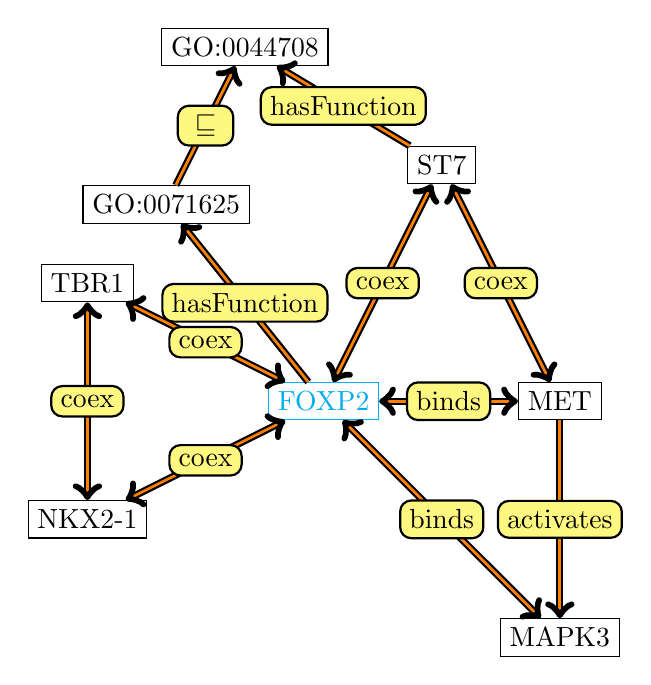
\begin{tikzpicture}
%          \SetUpEdge[lw = 1pt, color = black]
          \GraphInit[vstyle=Shade]
          \tikzset{
            LabelStyle/.style = { rectangle, rounded corners, draw,
              minimum width = 2em, fill = yellow!50,
              text = black },
            VertexStyle/.append style = { inner sep=5pt,
              font = \Large\bfseries},
            EdgeStyle/.append style = {->} }
          
          \SetGraphUnit{5}
          % \tikzset{VertexStyle/.append style={fill}}
          % \tikzset{EdgeStyle/.style={->}}
          \node[draw, color=cyan] (FOXP2) at (0,0) {FOXP2};
          \node[draw] (MET) at (3,0) {MET};
          \node[draw] (ST7) at (1.5,3) {ST7};
          \node[draw] (MAPK3) at (3,-3) {MAPK3};
          \node[draw] (GO0071625) at (-2,2.5) {GO:0071625};
          \node[draw] (GO0044708) at (-1,4.5) {GO:0044708};
          \node[draw] (TBR1) at (-3,1.5) {TBR1};
          \node[draw] (NKX2-1) at (-3,-1.5) {NKX2-1};
          \begin{scope}[/tikz/handle active characters in nodes=false]
          \Edge[label=activates](MET)(MAPK3)
          \Edge[label=hasFunction](FOXP2)(GO0071625)
          \Edge[label=hasFunction](ST7)(GO0044708)
          \Edge[label=$\sqsubseteq$](GO0071625)(GO0044708)

          \tikzset{EdgeStyle/.append style={<->}}
          \Edge[label=binds](FOXP2)(MET)
          \Edge[label=binds](FOXP2)(MAPK3)
          \Edge[label=coex](FOXP2)(TBR1)
          \Edge[label=coex](FOXP2)(NKX2-1)
          \Edge[label=coex](FOXP2)(ST7)
          \Edge[label=coex](MET)(ST7)
          \Edge[label=coex](NKX2-1)(TBR1)
          \end{scope}
          % \tikzset{EdgeStyle/.style={->}}
          % \Edge[label=hf](FOXP2)(GO0044708)
          % \draw[label=binds] (FOXP2) to (MET);
          % \Edge[label=binds](FOXP2)(MET)
          % \Edge[label=activates](MET)(MAPK3)
          % \Edge[label=coexpressed-with](FOXP2)(FOXP4)
          
        \end{tikzpicture}
      }
    \end{column}
    \begin{column}{.4\textwidth}
      \begin{itemize}
      \item task: predict if FOXP2 is involved in disease $D$
      \item task: what chemicals could (directly or indirectly) affect
        FOXP2's function?
      \item which features are relevant?
      \end{itemize}
    \end{column}
  \end{columns}
      
\end{frame}

\begin{frame}
  \frametitle{Neuro-symbolic feature learning}
  \begin{columns}
    \begin{column}{.6\textwidth}
      \resizebox{1\textwidth}{!}{%
        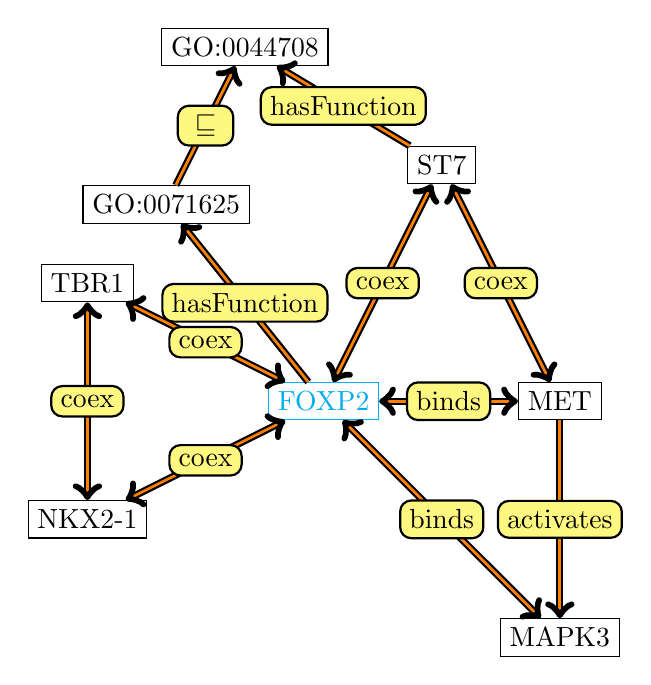
\begin{tikzpicture}
%          \SetUpEdge[lw = 1pt, color = black]
          \GraphInit[vstyle=Shade]
          \tikzset{
            LabelStyle/.style = { rectangle, rounded corners, draw,
              minimum width = 2em, fill = yellow!50,
              text = black },
            VertexStyle/.append style = { inner sep=5pt,
              font = \Large\bfseries},
            EdgeStyle/.append style = {->} }
          
          \SetGraphUnit{5}
          % \tikzset{VertexStyle/.append style={fill}}
          % \tikzset{EdgeStyle/.style={->}}
          \node[draw, color=cyan] (FOXP2) at (0,0) {FOXP2};
          \node[draw] (MET) at (3,0) {MET};
          \node[draw] (ST7) at (1.5,3) {ST7};
          \node[draw] (MAPK3) at (3,-3) {MAPK3};
          \node[draw] (GO0071625) at (-2,2.5) {GO:0071625};
          \node[draw] (GO0044708) at (-1,4.5) {GO:0044708};
          \node[draw] (TBR1) at (-3,1.5) {TBR1};
          \node[draw] (NKX2-1) at (-3,-1.5) {NKX2-1};
          \begin{scope}[/tikz/handle active characters in nodes=false]
          \Edge[label=activates](MET)(MAPK3)
          \Edge[label=hasFunction](FOXP2)(GO0071625)
          \Edge[label=hasFunction](ST7)(GO0044708)
          \Edge[label=$\sqsubseteq$](GO0071625)(GO0044708)

          \tikzset{EdgeStyle/.append style={<->}}
          \Edge[label=binds](FOXP2)(MET)
          \Edge[label=binds](FOXP2)(MAPK3)
          \Edge[label=coex](FOXP2)(TBR1)
          \Edge[label=coex](FOXP2)(NKX2-1)
          \Edge[label=coex](FOXP2)(ST7)
          \Edge[label=coex](MET)(ST7)
          \Edge[label=coex](NKX2-1)(TBR1)
          \end{scope}
          % \tikzset{EdgeStyle/.style={->}}
          % \Edge[label=hf](FOXP2)(GO0044708)
          % \draw[label=binds] (FOXP2) to (MET);
          % \Edge[label=binds](FOXP2)(MET)
          % \Edge[label=activates](MET)(MAPK3)
          % \Edge[label=coexpressed-with](FOXP2)(FOXP4)
          
        \end{tikzpicture}
      }
    \end{column}
    \begin{column}{.4\textwidth}
      % \begin{itemize}
      % \item task: predict if FOXP2 is involved in disease $D$
      % \item which features are relevant?
      %   \pause
      % \item learn relevant features $\Rightarrow$ knowledge graph
      %   embedding
      %   \pause
      % \item incorporate inferences by deductively closing the graph
      % \end{itemize}
    \end{column}
  \end{columns}
      
\end{frame}

\begin{frame}
  \frametitle{Neuro-symbolic feature learning}
  \begin{columns}
    \begin{column}{.6\textwidth}
      \resizebox{1\textwidth}{!}{%
        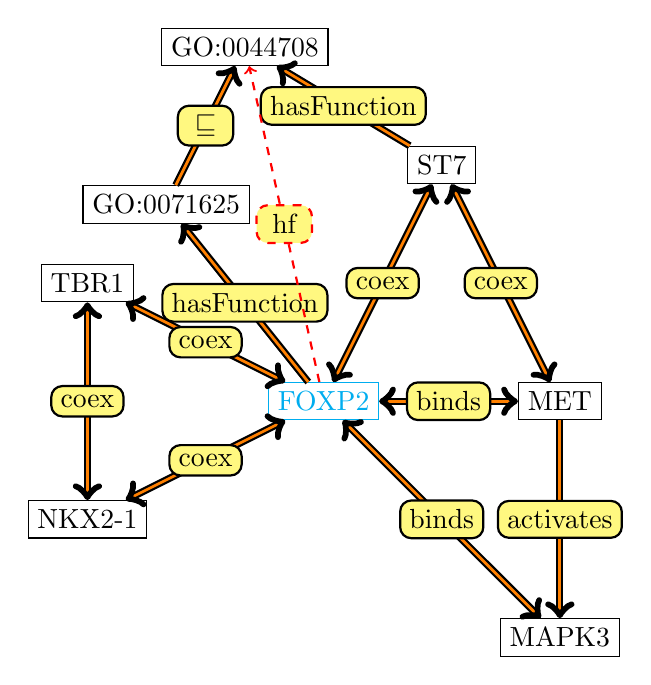
\begin{tikzpicture}
%          \SetUpEdge[lw = 1pt, color = black]
          \GraphInit[vstyle=Shade]
          \tikzset{
            LabelStyle/.style = { rectangle, rounded corners, draw,
              minimum width = 2em, fill = yellow!50,
              text = black },
            VertexStyle/.append style = { inner sep=5pt,
              font = \Large\bfseries},
            EdgeStyle/.append style = {->} }
          
          \SetGraphUnit{5}
          % \tikzset{VertexStyle/.append style={fill}}
          % \tikzset{EdgeStyle/.style={->}}
          \node[draw, color=cyan] (FOXP2) at (0,0) {FOXP2};
          \node[draw] (MET) at (3,0) {MET};
          \node[draw] (ST7) at (1.5,3) {ST7};
          \node[draw] (MAPK3) at (3,-3) {MAPK3};
          \node[draw] (GO0071625) at (-2,2.5) {GO:0071625};
          \node[draw] (GO0044708) at (-1,4.5) {GO:0044708};
          \node[draw] (TBR1) at (-3,1.5) {TBR1};
          \node[draw] (NKX2-1) at (-3,-1.5) {NKX2-1};
          \begin{scope}[/tikz/handle active characters in nodes=false]
          \Edge[label=activates](MET)(MAPK3)
          \Edge[label=hasFunction](FOXP2)(GO0071625)
          \Edge[label=hasFunction](ST7)(GO0044708)
          \Edge[label=$\sqsubseteq$](GO0071625)(GO0044708)

          \tikzset{EdgeStyle/.append style={<->}}
          \Edge[label=binds](FOXP2)(MET)
          \Edge[label=binds](FOXP2)(MAPK3)
          \Edge[label=coex](FOXP2)(TBR1)
          \Edge[label=coex](FOXP2)(NKX2-1)
          \Edge[label=coex](FOXP2)(ST7)
          \Edge[label=coex](MET)(ST7)
          \Edge[label=coex](NKX2-1)(TBR1)

          \tikzset{EdgeStyle/.style={->}}
          \Edge[label=hf, color=red, style=dashed](FOXP2)(GO0044708)
          \end{scope}
          % \draw[label=binds] (FOXP2) to (MET);
          % \Edge[label=binds](FOXP2)(MET)
          % \Edge[label=activates](MET)(MAPK3)
          % \Edge[label=coexpressed-with](FOXP2)(FOXP4)
          
        \end{tikzpicture}
      }
    \end{column}
    \begin{column}{.4\textwidth}
      \begin{itemize}
        \pause
      \item :FOXP2 :binds :MET :coex :ST7 :hasFunction GO:0044708
        \pause
      \item :FOXP2 :hasFunction GO:0071625 subClassOf GO:0044708
        \pause
      \item :FOXP2 :coex :TBR1 :coex :NKX2-1 :coex :TBR1 :coex ...
      \end{itemize}
    \end{column}
  \end{columns}
\end{frame}

\begin{frame}
  \frametitle{Neuro-symbolic feature learning}
  \begin{itemize}
  % \item iterated random walk from each node (in a knowledge graph
  %   consisting of instances and classes) defines sentences
  % \item one embedding for every node and edge type in our graph
  \item skip-gram model learns representation/features for each node
    \begin{itemize}
    \item Word2Vec model, given a word predicts context
    \item use local and non-local information
    \end{itemize}
  \item automated reasoning deductively closes the knowledge graph
    \begin{itemize}
    \item making this a neuro-symbolic model
    \end{itemize}
  \item useful for edge prediction, similarity, clustering, as feature
    vectors
    \begin{itemize}
    \item edge prediction: analogy, classifier (e.g., SVM)
    \end{itemize}
  \end{itemize}
\end{frame}

\begin{frame}
  \frametitle{Neuro-symbolic feature learning}
  \centerline{\includegraphics[width=\textwidth]{rdf-walking-datasets.png}}
\end{frame}

\begin{frame}
  \frametitle{Neuro-symbolic feature learning}
    \begin{table}[ht!]
  \resizebox{\textwidth}{!}{%
      \centering
      \begin{tabular}{@{}lllcccc@{}}\toprule 
        \multirow{2}{*}{Object property} 
        & Source type & Target type &\multicolumn{2}{c}{Without reasoning}&\multicolumn{2}{c}{With reasoning}\\
        &&& F-measure & AUC & F-measure & AUC \\
        \midrule
        has target & Drug & Gene/Protein & 0.94 & 0.97 & 0.94 & 0.98 \\
        has disease annotation & Gene/Protein & Disease & 0.89 & 0.95 & 0.89 & 0.95 \\
        has side-effect$^*$ & Drug & Phenotype & 0.86 & 0.93 & 0.87 & 0.94 \\
        has interaction & Gene/Protein & Gene/Protein & 0.82 & 0.88 & 0.82 & 0.88\\
        has function$^*$ & Gene/Protein & Function & 0.85 & 0.95 & 0.83 & 0.91 \\
        has gene phenotype$^*$  & Gene/Protein & Phenotype & 0.84 & 0.91 & 0.82 & 0.90  \\
        has indication & Drug & Disease & 0.72 & 0.79 & 0.76 & 0.83 \\
        has disease phenotype$^*$  & Disease & Phenotype & 0.72 & 0.78 & 0.70 & 0.77 \\
      \end{tabular}
  }
\end{table}
\vfill
{\tiny Alsharani et al. Neuro-symbolic representation learning on
biological knowledge graphs. Bioinformatics, 2017.}
\end{frame}

\begin{frame}
  \frametitle{Multi-modal feature learning}
    \begin{quote}
      The \only<1,2>{\underline{forkhead-box P2 (FOXP2)}}\only<3>{\underline{:FOXP2}} gene polymorphism has been
      reported to be involved in the susceptibility to schizophrenia;
      however, few studies have investigated the association between
      \only<1,2>{\underline{FOXP2}}\only<3>{\underline{:FOXP2}} gene polymorphism and clinical symptoms in schizophrenia.
    \end{quote}
  \pause
  \begin{itemize}
  \item \underline{:FOXP2} :binds :MET :coex :ST7 :hasFunction GO:0044708
  \item \underline{:FOXP2} :hasFunction GO:0071625 subClassOf GO:0044708
  \item \underline{:FOXP2} :coex :TBR1 :coex :NKX2-1 :coex :TBR1 :coex ...
  \end{itemize}
\end{frame}

\begin{frame}
  \frametitle{Multi-modal feature learning}
  \centerline{\includegraphics[width=\textwidth]{multimodal_workflow.pdf}}
\end{frame}


\begin{frame}
  \frametitle{Multi-modal feature learning: drug targets and indications}
  \centerline{
    \includegraphics[width=.45\textwidth]{DTI_ANN_all.pdf}
    \includegraphics[width=.45\textwidth]{Ind_ANN_all.pdf}
  }
  \vspace{.5cm}
  {\tiny Alshahrani \& H. Drug repurposing through
    multi-modal learning on knowledge graphs. BioRxiv, 2018.}
\end{frame}



\subsection{Translating embeddings}



\subsection{Syntactic approaches}

\begin{frame}
  \frametitle{Ontologies: axioms, not graphs!}
    \includegraphics[width=1\textwidth]{bcellapoptosis.png}
\end{frame}

\begin{frame}
  \frametitle{Ontologies: axioms, not graphs!}
  Gene Ontology:
  \begin{itemize}
  \item {\tt behavior DisjointWith: 'developmental process'}
  \item {\tt behavior SubclassOf: only-in-taxon some metazoa}
  \item {\tt 'cell proliferation' DisjointWith: in-taxon some fungi}
  \item {\tt 'cell growth' EquivalentTo: growth and ('results in
      growth of' some cell)}
  \item ...
  \end{itemize}
\end{frame}

% \begin{frame}
%   \frametitle{Ontologies: axioms, not graphs!}
%   \begin{itemize}
%   \item converting ontologies to graphs
%     \begin{itemize}
%     \item loses information
%     \end{itemize}
%   \item relations between ontologies
%   \end{itemize}
% \end{frame}

\begin{frame}
  \frametitle{Ontology embeddings}
  \begin{definition}
    Let $O = (C, R, I; ax; \vdash)$ be an ontology with a set of
    classes $C$, a set of relations $R$, a set of instances $I$, a set
    of axioms $ax$ and an inference relation $\vdash$. An ontology
    embedding is a function $f_\eta : C \cup R \cup I \mapsto
    \mathbf{R}^n$ (subject to certain constraints).
  \end{definition}
  \pause For example, we can use co-occurrence within $ax^\vdash$ to
  constrain the embedding function, where the constraints on
  co-occurrence are formulated using the Word2Vec skipgram model.
\end{frame}

\begin{frame}
  \frametitle{Onto2Vec}
  \centerline{\includegraphics[width=\textwidth]{onto2vecflow.png}}
\end{frame}

\begin{frame}
  \frametitle{Predicting PPIs: trainable similarity measures}
  \centerline{\includegraphics[width=.45\textwidth]{YSTUnsuper1.png}\includegraphics[width=.45\textwidth]{YstUnsup2.png}}
  \vfill
  {\tiny Smaili et al. Onto2Vec: joint vector-based representation of
    biological entities and their ontology-based annotations, Bioinformatics, 2018.}
\end{frame}

\begin{frame}
  \frametitle{Visualizing embeddings}
  \centerline{\includegraphics[width=.9\textwidth]{updtsne.jpg}}
\end{frame}

\begin{frame}
  \frametitle{Ontologies Plus Annotations 2 Vec}
  \centerline{\includegraphics[width=1\textwidth]{opaworkflow16.png}}
\end{frame}

\begin{frame}
  \frametitle{Phenotype-based prediction of candidate genes}
  \centerline{
    \includegraphics[width=.45\textwidth]{Human_Disease.png}
    \includegraphics[width=.45\textwidth]{HD.png}
  }
\end{frame}


\subsection{Model-theoretic approaches}

\begin{frame}
  \frametitle{Description Logic EL++}
  \centering
  \resizebox{.8\textwidth}{!}{
    
    \begin{tabular}{|p{1.7cm}|c|p{3.7cm}|}
      \hline
      {\bf} Name & Syntax & Semantics \\
      \hline
      top & $\top$ & $\Delta^{\mathcal{I}}$ \\
    \hline
    bottom & $\bot$ & $\emptyset$ \\
    \hline
    nominal & $\{ a \} $ & $\{ a^{\mathcal{I}} \}$ \\
    \hline
    conjunction & $C \sqcap D$ & $ C^{\mathcal{I}} \cap
                                 D^{\mathcal{I}}$ \\
    \hline
    existential restriction & $\exists r.C$ & $ \{ x \in
                                              \Delta^{\mathcal{I}} |
                                              \exists y \in
                                              \Delta^{\mathcal{I}} :
                                              (x,y) \in
                                              r^{\mathcal{I}} \land y
                                              \in C^{\mathcal{I}} \} $
    \\
    \hline
    generalized concept inclusion & $C \sqsubseteq D$ &
                                                        $C^{\mathcal{I}}
                                                        \subseteq
                                                        D^{\mathcal{I}}$
    \\
    \hline
    role inclusion & $r_1 \circ ... \circ r_n \sqsubseteq r$ &
                                                               $r_1^{\mathcal{I}}
                                                               \circ
                                                               ... \circ
                                                               r_n^{\mathcal{I}}
                                                               \subseteq
                                                               r^{\mathcal{I}}$
    \\
    \hline
    
  \end{tabular}
}
\end{frame}

\begin{frame}
  \frametitle{EL Embeddings}
  \begin{itemize}
  \item aim: given an EL++ theory $T$, find $f_e: T \mapsto
    \mathbb{R}^n$ s.t. $f_e(T)$ is a model of $T$ ($f_e(T) \models T$)
    \pause
  \item any consistent EL++ theory has models in $\mathbb{R}^n$
    (Loewenheim-Skolem, upwards)
    \pause
  \item key idea:
    \begin{itemize}
    \item for all $r \in \Sigma(T)$ and $C \in \Sigma(T)$, define
      $f_e(r)$ and $f_e(C)$
    \item $f_e(C)$ maps to points in an open $n$-ball such that
      $f_e(C) = C^{\mathcal{I}}$:
      $C^{\mathcal{I}} = \{ x \in \mathbb{R}^n | \norm{f_e(C) - x} <
      r_e(C) \}$
    \item $f_e(r)$ maps a binary relation $r$ to a vector such that
      % the set of tuples ($\mathbb{R}^n \times \mathbb{R}^n$) with
      % $f_e(r) = r^{\mathcal{I}}$:
      $r^{\mathcal{I}} = \{ (x,y) | x + f_e(r) = y \}$
    \item use the axioms in $T$ as constraints
    \end{itemize}
  \end{itemize}
\end{frame}

\begin{frame}
  \frametitle{EL Embeddings}
  \centerline{\animategraphics[loop,controls,width=.7\textwidth]{12}{embeds-frame-}{0}{99}}
  \begin{itemize}
  \item model with $\Delta = R^n$
  \item support quantifiers, negation, conjunction,...
  \end{itemize}
  {\tiny IJCAI 2019}
\end{frame}



% \begin{frame}
%   \frametitle{Hands-on part}
%   \begin{itemize}
%   \item run the machine learning with ontologies part
%   \item explore the different similarity measures
%   \item repeat what you have done with semantic similarity using the
%     ontology embeddings
%   \end{itemize}
% \end{frame}

\begin{frame}
  \frametitle{How to measure similarity?}
  \begin{itemize}
  \item vector-based similarity measure
  \item cosine similarity: $sim(X,Y) = \frac{\sum_{i=1}^n X_i
      Y_i}{\sqrt{\sum_{i=1}^n X_i^2} \sqrt{\sum_{i=1}^n Y_i^2}} $
    \begin{itemize}
    \item bounded between $[-1,1]$
    \end{itemize}
  \item Euclidean distance: $sim(X,Y) = \sqrt{\sum_{i=1}^n (X_i - Y_i)^2}$
    \begin{itemize}
    \item not bounded (and rarely used)
    \end{itemize}
  \item any other kind of function
    \begin{itemize}
    \item Neural Networks can approximate {\em any} function
      (universal approximation theorem)
    \item ``trainable'' semantic similarity measures
    \item will need training data
    \end{itemize}
  \end{itemize}
\end{frame}

\section{Applications}


\begin{frame}
  \frametitle{Applications of semantic similarity}
  \centerline{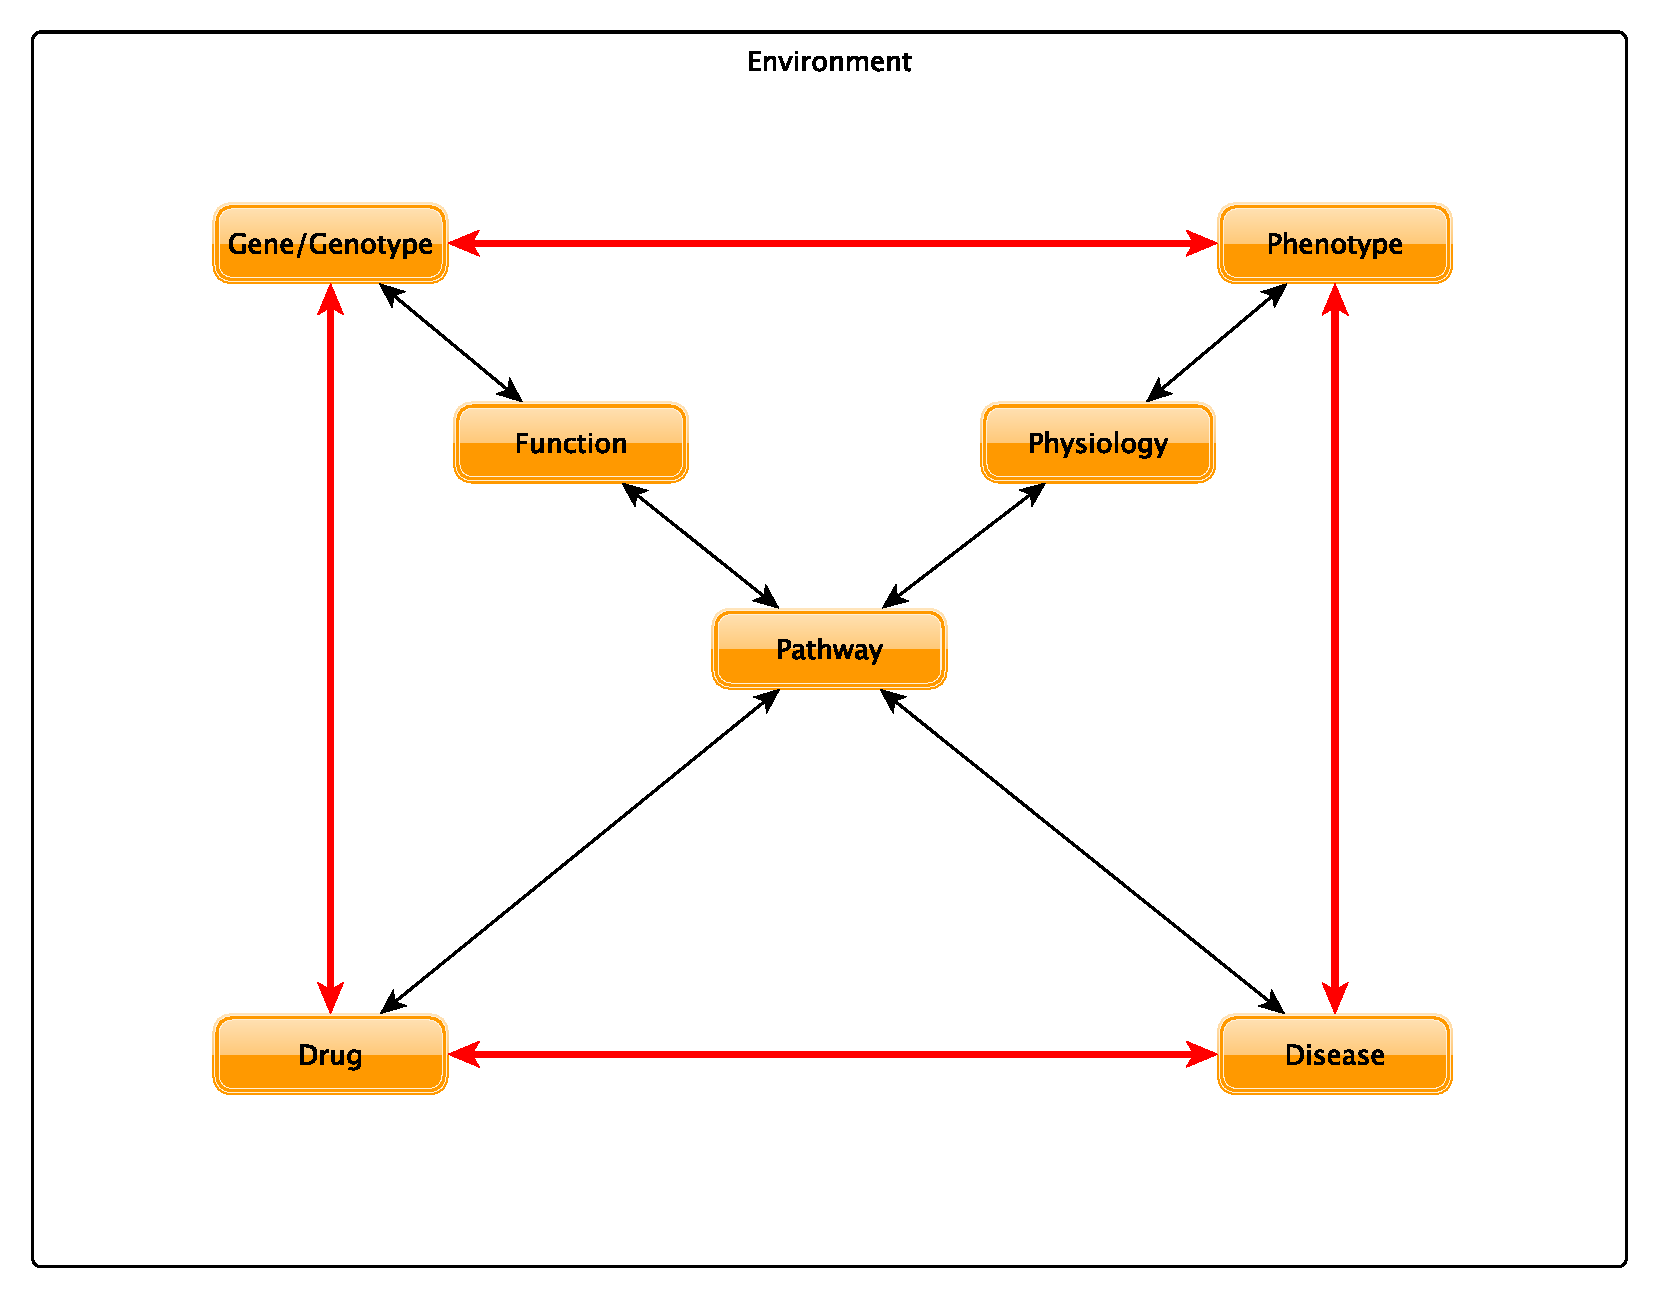
\includegraphics[height=\textheight]{vision1.pdf}}
\end{frame}

\begin{frame}
  \frametitle{Applications of semantic similarity}
  \centerline{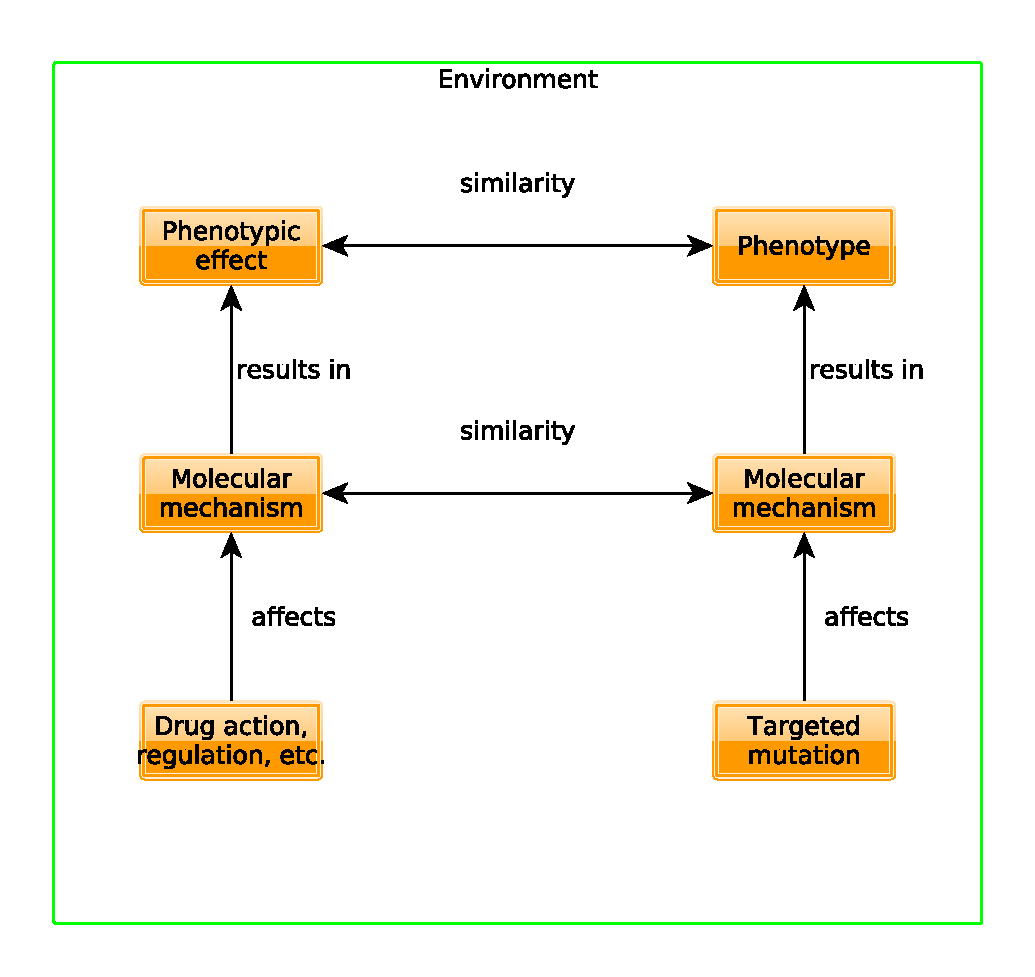
\includegraphics[height=\textheight]{similarity.eps}}
\end{frame}

\begin{frame}
  \frametitle{Applications of semantic similarity}
  \begin{itemize}
  \item same kind of entity, same ontology:
    \begin{itemize}
    \item $x$ is associated with $y$
    \item $z$ is similar to $x$
    \item therefore: $z$ may {\em also} be associated with $y$
    \end{itemize}
  \item candidate genes (polygenic disease):
    \begin{itemize}
    \item FunSimMat: similar function $\Rightarrow$ similar/same
      disease
    \item side effect similarity: similar side effects $\Rightarrow$
      similar targets/indications
    \end{itemize}
  \end{itemize}
\end{frame}

\begin{frame}
  \frametitle{Applications of semantic similarity}
  \begin{itemize}
  \item different kind of entity, same ontology:
%  \item candidate genes (monogenic and polygenic disease):
    \begin{itemize}
    \item Phenomizer: genotype $x$ associated with phenotypes $a$;
      patient $y$ has symptoms $b$; $a$ is similar to $b$; therefore:
      $x$ causes the symptoms in $b$
    \item PhenomeNET: similar to Phenomizer but using model organism
      phenotypes (knockouts)
    \item PhenomeDrug: knockout of gene $x$ causes phenotypes $a$;
      drug $y$ causes side effects $b$; $a$ is similar to $b$;
      therefore: drug $y$ inhibits $x$ (or: phenotypes $b$ are caused
      by inhibition of $x$)
    \item needs to compare model organism phenotypes and human
      phenotypes $\Rightarrow$ ontology alignment/integration/mapping
    \end{itemize}
  \end{itemize}
\end{frame}

% \begin{frame}
%   \frametitle{Applications of semantic similarity}
%   semantic similarity and text mining:
%   \begin{itemize}
%   \item find all occurrences of classes of one (or more) ontologies in text
%     \begin{itemize}
%     \item using lexical matching or semantic annotations
%       of text
%     \item TextPresso (\url{http://www.textpresso.org/}), NCBO
%       Annotator (\url{https://bioportal.bioontology.org/annotator}),
%       WhatIzIt (\url{http://www.ebi.ac.uk/webservices/whatizit/info.jsf})
%     \item ontology-specific text normalization tools
%       \begin{itemize}
%       \item DNorm (diseases), GNorm (gene names), OSCAR (chemicals), ...
%       \end{itemize}
%     \end{itemize}
%   \item use for database construction (automatic annotation), relation
%     extraction, network construction (co-occurrence network), etc.
%   \end{itemize}
% \end{frame}

% \begin{frame}
%   \frametitle{Applications of semantic similarity}
%   \centerline{http://aber-owl.net/aber-owl/diseasephenotypes/}
%   \begin{itemize}
%   \item find phenotypes (signs and symptoms) associated with common
%     diseases
%     \begin{itemize}
%     \item no resource available for comparison
%     \end{itemize}
%   \item pattern-based mining of literature with Aber-OWL: PubMed
%   \item evaluation (of genetically based disease phenotypes) with
%     experimentally validated disease genes
%   \end{itemize}
% \end{frame}

% \begin{frame}
%   \frametitle{Applications of semantic similarity}
%   \framesubtitle{http://aber-owl.net/aber-owl/diseasephenotypes/}
%   \centerline{\includegraphics[width=1\textwidth]{aber-owl-plague.png}}
% \end{frame}

% \begin{frame}
%   \frametitle{Applications of semantic similarity}
%   \framesubtitle{http://aber-owl.net/aber-owl/diseasephenotypes/}
%   \centerline{\includegraphics[width=1\textwidth]{pmi-auc-plot.pdf}}
% \end{frame}

% \begin{frame}[plain]
%   \frametitle{Applications of semantic similarity}
%   \centerline{\includegraphics[height=1\textheight]{network.eps}}
% \end{frame}

% \begin{frame}
%   \frametitle{Applications of semantic similarity}
%   \begin{itemize}
%   \item semantic similarity can be used as features in machine
%     learning models
%     \begin{itemize}
%     \item when annotation space is too large
%       \begin{itemize}
%       \item e.g., GO: 50,000 classes
%       \item replace binary representation
%       \end{itemize}
%     \item to incorporate background knowledge
%       \begin{itemize}
%       \item semantic similarity encodes {\em implicitly} for ontology
%         structure and axioms
%       \item encodes for {\em specificity} of classes
%       \end{itemize}
%     \item negative: reduce all annotations to single value
%       \begin{itemize}
%       \item leads to loss of information
%       \item but is easier to use by many machine learning methods
%       \end{itemize}
%     \end{itemize}
%   \end{itemize}
% \end{frame}

% \begin{frame}
%   \frametitle{Applications of semantic similarity}
%   \begin{tikzpicture}[remember picture,overlay]
%     \node[at=(current page.center)] {
%       \centerline{\includegraphics[height=1\textheight]{pvp.pdf}}
%     };
%   \end{tikzpicture}
% \end{frame}

% {
% \setbeamercolor{background canvas}{bg=}
% \includepdf[pages=1-3]{hh-pvp2.pdf}
% }

% \begin{frame}
%   \frametitle{Summary}
%   \begin{itemize}
%   \item many semantic similarity measures
%     \begin{itemize}
%     \item graph-based
%     \item feature-based
%     \end{itemize}
%   \item useful for similarity-based prediction
%     \begin{itemize}
%     \item similar entities $\Rightarrow$ guilt-by-association
%     \item different entities
%     \end{itemize}
%   \item combine with data and text mining
%   \item features in machine learning methods
%   \end{itemize}
% \end{frame}

% \begin{frame}
%   \frametitle{Acknowledgements}
%   \begin{itemize}
%   \item Sarah Alghamdi
%   \item Mona Alsharani
%   \item Imene Boudellioua
%   \item Senay Kafkas
%   \item Maxat Kulmanov
%   \item Fatima Zohra Smaili
%   \end{itemize}
% \end{frame}

\begin{frame}
  \frametitle{Hands-on: semantic similarity}
  \begin{itemize}
  \item if you have not done so {\em before} the tutorial, don't start
    now
    \begin{itemize}
    \item you need to download {\em a lot} of data
    \item you can just follow our demonstration and try later
    \item (unless Internet is exceptionally fast for a conference
      Wifi, then just go ahead and do everything now)
    \end{itemize}
  \item Jupyter Notebook
    \begin{itemize}
    \item notebooks consist of code and rich text fragments
    \item human readable (with nice figures) {\em and} executable
    \item need to install the SciJava kernel (default: iPython)
    \item very widely used
    \end{itemize}
  \item
    \url{https://github.com/bio-ontology-research-group/ontology-tutorial}
  \end{itemize}
\end{frame}

\begin{frame}
  \frametitle{Hands-on: semantic similarity}
  In the tutorial, we will
  \begin{itemize}
  \item download an ontology
  \item explore the ontology with OWLAPI
  \item classify the ontology with an OWL reasoner
    \begin{itemize}
    \item and query using an OWL reasoner
    \end{itemize}
  \item store the inferred version locally
  \item use the Semantic Measures Library to:
    \begin{itemize}
    \item explore the ontology as graph
    \item compute similarity between classes
    \item use different similarity measures
    \item compare patients to mice
    \end{itemize}
  \item learn to use Onto2Vec and OPA2Vec
  \item you can build on this and extend for your own research!
  \end{itemize}
\end{frame}

\begin{frame}
  \frametitle{Hands-on: semantic similarity}
  Do the tutorial...
\end{frame}

\begin{frame}
  \frametitle{Hands-on: semantic similarity}
  \begin{itemize}
  \item now play with the Notebook:
    \begin{itemize}
    \item look at the results list (check MGI)
    \item try another disease (check OMIM)
    \item or a drug effect (check SIDER)
    \end{itemize}
  \item you can also test another ontology
    \begin{itemize}
    \item GO for functional similarity
    \item ChEBI for chemical (structural) similarity
    \item or yeast phenotypes
    \end{itemize}
  \end{itemize}
\end{frame}

\end{document}
%%% Local Variables:
%%% mode: latex
%%% TeX-master: t
%%% End:
